\documentclass[sigplan]{acmart}

\usepackage{booktabs}
\usepackage{graphicx}
\usepackage{amsmath}
\usepackage{hyperref}
%\usepackage[font=bf]{caption}
\usepackage{caption}
\usepackage{subcaption}
\usepackage{algorithm}
\usepackage{algpseudocode}
\usepackage{graphicx}
\usepackage{booktabs}
\usepackage{color}
\usepackage{ifthen}
\usepackage{flushend}
\newcommand{\cL}{{\cal L}}

\newcommand{\tmem}{\textrm{tmem}}
\newcommand{\get}{\textrm{get}}
\renewcommand{\put}{\textrm{put}}
\newcommand{\flush}{\textrm{flush}}
\newcommand{\cleancache}{\textrm{cleancache}}
\newcommand{\gh}{\textrm{G-H}}
\newcommand{\dd} {\textrm{DoubleDecker}}
\newcommand{\web} {\textrm{Webserver}}
\newcommand{\proxy} {\textrm{Proxycache}}
\newcommand{\mail} {\textrm{Mail}}
\newcommand{\video} {\textrm{Videoserver}}
\newcommand{\file} {\textrm{Filebench}}
\newcommand{\zcache} {\textrm{zcache}}
\newcommand{\cgroup} {\textrm{Cgroup}}
\newcommand{\cgroups} {\textrm{Cgroups}}

\newcommand{\puru}[1]{\textcolor{red}{[Puru: #1]}}
\newcommand{\deba}[1]{\textcolor{red}{[Deba: #1]}}
\newcommand{\revised}[1]{\textcolor{magenta}{#1}}
\sloppy
\copyrightyear{2017} 
\acmYear{2017} 
\setcopyright{acmcopyright}
\acmConference{Middleware '17}{December 11--15, 2017}{Las Vegas, NV,
USA}
\acmPrice{15.00}
\acmDOI{https://doi.org/10.1145/3135974.3135992}
\acmISBN{978-1-4503-4720-4/17/12}


\begin{document}

%\title{DoubleDecker: A Quasi-decentralized Memory Management Framework for Derivative Clouds}
% \title{DoubleDecker: A cooperative memory management framework for derivative clouds}
\title{DoubleDecker: A cooperative disk caching framework for derivative clouds}
\author{Debadatta Mishra}
\authornote{Work done when the author was a student at IIT Bombay}
\affiliation{%
  \institution{Indian Institute of Technology Kanpur}
%  \state{Kanpur, India} 
}
\email{deba@cse.iitk.ac.in}


\author{Prashanth}
\affiliation{%
  \institution{Indian Institute of Technology Bombay}
%  \state{Mumbai, India} 
}
\email{prashanth@cse.iitb.ac.in}

\author{Purushottam Kulkarni}
\affiliation{%
  \institution{Indian Institute of Technology Bombay}
%  \state{Mumbai, India} 
}
\email{puru@cse.iitb.ac.in}

\settopmatter{printacmref=true, printccs=true, printfolios=false}
\setcopyright{acmcopyright}

%abstract.tex
\begin{abstract}
Derivative clouds, light weight application containers provisioned
in virtual machines, are becoming viable and cost-effective
options for infrastructure and software-based services.
%Iaas and PaaS services.
%Derivative clouds, a recent IaaS/PaaS service delivery mechanism,
%is becoming popular due to its support for business model flexibility
%in a cost effective manner.
%
%In this model, lightweight application containers are provisioned in 
%virtual machines (VMs) to provide an application platforms for the end 
%customers.
%
%State-of-the-art hypervisors and application container isolation 
%frameworks are not designed to integrate in a seamless manner. 
%
%This is specifically prominent in the resource management procedures.
%where there is no handshake between the two entities to determine and 
%enforce resource management policies.
%
%to provide
%clear resource management boundaries---at system level by the hypervisors
%and at a per-VM level by the guest administrator.
%
Ubiquitous dynamic memory management techniques in virtualized systems 
are centralized at the hypervisor %which may not be as 
and are ineffective
in nested derivative cloud setups.
%
%work propose to push the decision ma
%
In this paper, we highlight the challenges in management of 
memory resources in derivative cloud systems.
%hypervisor based second-chance cache for virtual machines in 
%(acting as a second chance cache for VMs) in derivative 
%cloud (nested) systems.
%
Hypervisor caching, an enabler of centralized disk cache management,
provides flexible memory or non-volatile memory management at the hypervisor 
to improve the resource usage efficiency and performance of applications.
%at the system level.
%
%However, hypervisor caches have no support for multi-level differentiated 
%provisioning, and therefore are not directly adaptable in 
%a derivative cloud setup.
Existing hypervisor caching solutions have limited effectiveness in 
nested setups due to their nesting agnostic design, centralized 
management model and lack of holistic view of memory management.
%
We propose \dd{}, a decentralized disk caching framework,
%memory management framework,
realized through guest OS and hypervisor cooperation,
with support for efficient memory management in derivative clouds.
%
The \dd{} hypervisor caching framework, an integral part of our proposed solution,
provides interfaces for differentiated cache partitioning and management in 
nested setups and is equipped to handle both memory and SSD based caching stores.
%to apply inter-VM and intra-VM
%(application) level 
%
We demonstrate the flexibility of \dd{} to handle dynamic and
changing memory provisioning requirements and 
its capability to simultaneously provision memory
across multiple levels.
%
Such multi-level configurations cannot be explored by centralized designs
and are a key feature of \dd{}.
%distinguish the enhanced feature set enabled by \dd{} for
%improved memory management decisions.
%and its efficacy in designing holistic policies confirming to 
%multi-level policy objectives.
%
Our experimentation with \dd{} demonstrates
that application performance
can be consistently improved due to the
flexible policy framework for disk caching.
% extended set of
%memory provisioning configurations. 
With our setup, we report an average
performance improvement of 4x and a maximum of 11x.
%
%improved by up to 11 times compared to application agnostic
%provisioning techniques.
%... \puru{add a
%couple of high level results here.}
%By extending the application container level relative
%weights to the hypervisor cache, \dd{} could improve the 
%application performance by up to 11 times. 
%With selective
%provisioning applications to the SSD cache we demonstrate
%system-wide benefits.
\end{abstract}


 \begin{CCSXML}
<ccs2012>
<concept>
<concept_id>10011007.10010940.10010941.10010942.10010948</concept_id>
<concept_desc>Software and its engineering~Virtual machines</concept_desc>
<concept_significance>500</concept_significance>
</concept>
<concept>
<concept_id>10011007.10010940.10010941.10010949.10010950</concept_id>
<concept_desc>Software and its engineering~Memory management</concept_desc>
<concept_significance>500</concept_significance>
</concept>
<concept>
<concept_id>10011007.10010940.10010971.10011120.10003100</concept_id>
<concept_desc>Software and its engineering~Cloud computing</concept_desc>
<concept_significance>500</concept_significance>
</concept>
</ccs2012>
\end{CCSXML}

\ccsdesc[500]{Software and its engineering~Virtual machines}
\ccsdesc[500]{Software and its engineering~Memory management}
\ccsdesc[500]{Software and its engineering~Cloud computing}

\maketitle


\section{Introduction}
\label{sec:intro}

A vital enabler for high consolidation ratios of virtual machines
in virtualization based hosting platforms
is memory overcommitment~\cite{vmware,vmware:memory}. 
%
The key idea of techniques relying on
overcommitment is to exploit the tradeoff between
dynamic memory provisioning and usage efficiency, and 
performance implications.
%
%Efficient memory management in virtualized
%systems enables increased virtual machine {\em consolidation density} 
%through higher levels of memory utilization.
%
%where at the system level hypervisors are agnostic of the nesting
%and guest operating systems have no defined interfaces for 
%providing information for explicit container-level resource
%provisioning.
%Increased memory efficiency results in higher levels of hardware
%availability and cost efficiency in terms of hardware,
%maintenance and power.
%
%Additional software layers in systems hosting multiple isolated execution 
%domains---hypervisors in virtualized systems~\cite{xen,kvm,vmware}, and,
%hypervisors and/or container 
%frameworks in nested virtualized systems~\cite{cgroup,docker,lxc}---present 
%several challenges in efficient resource management.
%
The challenge of memory management in virtualized systems~\cite{xen,kvm,vmware}
and container-based systems~\cite{cgroup,docker,lxc} is 
the opaqueness between the resource manager (the hypervisor or
the host operating system) and the resource user (guest operating
systems or applications).
%
%One of the main bottlenecks in these systems is the increased 
%opaqueness between the resource manager (hypervisor) and 
%the resource user (applications).
%
Techniques like dynamic ballooning~\cite{vmware,hotplug}, memory
content deduplication~\cite{vmware,ksmpaper} and hypervisor 
caching~\cite{memtrans,oracletmem,kvmzcache, geiger} 
%address the challenges by enabling 
enable dynamic provisioning, increased memory efficiency and 
system level disk cache provisioning for efficient memory 
management. % in virtualized systems.
%
While these techniques and associated policies have been studied
extensively in virtualization setups~\cite{vmware, membal, membud, kvmzcache, tws},
they have not been studied in \emph{nested hosting} setups.
\revised{
The central proposition of this work is that resource management
techniques employed with single-level virtualization setups
are inadequate in the context of nested-hosting setups 
and require augmentation and re-design.}

\revised{
%Additional overheads due to nested virtualization layers~\cite{blanket,turtle}
Overcoming the additional overheads due to nesting~\cite{blanket,turtle}
has been one of the primary bottlenecks in realizing sub-tenancy
models of cloud infrastructure services.
%
%Resource provisioning issues in nested settings gained less attention 
%because of the additional virtualization overheads~\cite{blanker,turtule} 
%in nested virtualization solutions discouraged its usage for enabling 
%cloud infrastructure services.
%
Provisioning of one or more application containers inside VMs, 
a recently popular nested hosting technique, has promising potential considering 
low virtualization overheads compared
to nesting virtual machines~\cite{middleware16,vmw-docker}. 
%
%Containers inside VMs enable subletting business models 
%like \emph{derivative cloud} model~\cite{spotcheck, google} which 
%is the focus of this work.
%
The \emph{derivative cloud} model~\cite{spotcheck, google}
instantiated with containers inside VMs is the focus of this work.
%
In the derivative model, an intermediate service provider builds
service offerings using services rented, leased or purchased.
%
The services themselves could be smaller sized versions of the
first-level service or could be applications, and in general host
other software-as-a-service or platform-as-a-service variants.
%
From the memory management perspective, with container based
derivative clouds, the container-based nested services
are provisioned and managed from within a virtual machine
and resources for virtual machines are managed by the 
hypervisor-level policy tools.
%
The notion of two isolated resource management entities with 
different levels of visibility into their respective managed 
components---containers at the virtual machine level and VMs at the
hypervisor level, require careful analysis of design alternatives.} 
%
%Containers are provisioned and managed by the VM administrators,
%who may want to employ higher level QoS policies in terms of priority or
%optimize the resource utilization depending on the application 
%characteristics.
%
%For VMs enabled with hypervisor caches, the differentiated partitioning
%Nested virtualization, recently popularized by application containers and 
%{\em Derivative clouds}~\cite{spotcheck,google}, enables hosting 
%application containers inside VMs.
%
%ballooning, deduplication and hypervisor caching is required to be 
%to analyze
%effectiveness in a nested virtualization setup.
%nested virtualization framework to analyze their 
%

\revised{
%In this work, our focus is the use of hypervisor caching for
%effective disk cache memory management in derivative clouds.
%the focus is to explore the hypervisor caching solution space 
%in nested hosting setups (containers inside VMs) and work out suitable 
%enhancements to enable efficient hypervisor caching for nested application 
%containers inside VMs.
%
%Memory used to cache disk content (a.k.a. page cache) can be
%a major bottleneck for efficient memory management in virtualized
%systems.
Memory used to cache disk content is a significant part of the 
system memory and its management in multi-hosting setups is
non-trivial.  
%
%Utility of a disk cache depends on application access behavior,
%e.g., access patterns (sequential vs. random) and read-write ratios.
%
%Best effort disk caches employed by 
Operating systems greedily consume
all available free memory in the system (and in a virtual machine)
to provision disk cache memory.
%, which may be wasteful in a multi-hosting scenario.  
%
Further, disk cache management decisions of a guest OS are 
localized to the virtual machine and are oblivious to memory 
usage and disk cache utility 
across the virtual machines hosted on the same physical machine.
}
%
%So, in a multi-hosting system, memory used to cache disk content 
%by applications (or operating systems), if managed
%at the system level, provide flexibility of differentiated 
%partitioning to meet system level objectives like
%application priority, cache utility etc..
%
Hypervisor caching~\cite{memtrans, oracletmem, kvmzcache, vmmexclusive, singleton} 
provides a mechanism for system-wide management of % to globally manage 
disk cache memory in virtualized systems. 
%
Hypervisor caches can be setup and used 
in two different configurations.
%
First, available free system memory can be used to setup a 
hypervisor managed second-chance cache.
%
Size of the second-chance cache and per-VM partitioning 
can be implemented based on resource management policies.
%provisioned dynamically 
%across virtual machines depending on higher level policies.
%
Second, dynamic adjustment of virtual machine memory allocations through
techniques like ballooning~\cite{vmware,hotplug} can explicitly
push the disk caching to the hypervisor, fully or partially.
%to enable system level management of memory use for disk content caching.
%
\deba{remove?
In fact, in the second configuration, the page cache of guest OSes
can be completely offloaded to the hypervisor.} 
%
The hypervisor in-turn can improve
memory efficiency by employing per-VM differentiated provisioning,
perform in-band compression and deduplication etc.~\cite{oracletmem,kvmzcache}.
%State-of-the-art hypervisor caching solutions---Xen Transcendent memory~\cite{oracletmem}and KVM compressed host cache ~\cite{kvmzcache}---provide mechanisms to
%distribute the hypervisor cache across VMs depending on
%high level objectives like VM priority and cache utility.
%

Applicability of hypervisor caching in a derivative cloud setup is 
hindered due to several reasons. Firstly, hypervisor cache management 
is agnostic to the execution entities within the virtual machine. 
For example, hypervisor caches cannot provide differential cache 
allocations to multiple applications executing within a virtual machine
in a seamless manner.
%
Enlightening the hypervisor cache with application level information 
as an alternative design is cumbersome and requires understanding and 
redesigning of the current integration framework. 
%
Secondly, in a derivative setup it may be useful for
guest OSes to holistically manage all memory resources---allocated
virtual machine memory and the hypervisor cache.
%
The current hypervisor caching solutions lack the capability to 
expose interfaces 
to provide visibility and local provisioning capability to the guest OS. 
%
%Secondly, the centralized model of hypervisor cache management 
%does not have the necessary artifacts to support {\em decentralized 
%policy enforcement requirements} of a derivative cloud.
%
%More specifically, with derivative
%clouds current hypervisor differentiated provisioning techniques
%cannot be extended to the nested entities due to the semantic
%barrier between the hypervisor and execution entities
%within virtual machines.
%partitioning at a finer granularity
%(e.g., at application level) is {\em not possible} in the existing 
%framework.
%
%This is because, hypervisor caches operate in an application
%agnostic manner and are unaware of application semantics due to the 
%opaque nature of applications with respect to the hypervisor caches.
%
%
%Thirdly, in a derivative cloud, memory management of applications
%inside a VM (containers) are not limited to only disk cache provisioning.
%



%Our analysis of employing hypervisor cache in a derivative cloud
%provides some interesting observations---hypervisor
%cognizance does not need to extend to applications if a handshake
%take cognizance of containers and still operate in an application
%agnostic manner. 
%
%An usage scenario would involve differentiated provisioning
%of the cache on a per-VM basis and the per-VM cache
%would be differentiated on a per-container basis.
%
A desired memory management model in derivative clouds is to
provide {\em independent memory management} at each level,
without non-deterministic side effects and without loss of
hypervisor control.
%{\em without
%encroaching} on each other.
%
The provisioning policies at each level should be mutually
exclusive and at the same time allow each hosting entity
to influence the memory provisioning decisions.
%
For example, a hypervisor level policy can be used to 
implement VM level priorities and application level priorities 
may be configured within each VM for differential treatment
for provisioning the VM-specific hypervisor cache. 
%of applications at the hypervisor level.
%
%puru commmented the next two lines
%This design allows a VM-level memory manager to
%enforce comprehensive policies beyond the hypervisor cache 
%provisioning.
%
%For example, a VM-level policy has the flexibility to meet
%application performance by provisioning in-VM memory and the
%hypervisor cache resources.  
%
\revised{
Our proposed solution addresses the above requirements 
through synergistic extensions in the guest OS
and the hypervisor. 
%
%We believe effectiveness of black-box techniques, as an alternate
%solution approach, would be bottlenecked because of two
%primary factors.
%
While a non-intrusive black box technique is a possibility,
it would require virtual machine transparent mechanisms to
identify containers and their memory usage behaviors.
%
Further, influencing guest OS memory management can be at best
influenced in an indirect manner, for which the cost-benefit
tradeoff can be prohibitive.
%
%can be performed
%in an indirect manner (if at all) which may not be as effective.
%
Moreover, given the struggle of black-box techniques 
to meet dynamic resource demands even in non-nested settings~\cite{vmware,membal}, 
we preferred a cooperative approach to address the above 
resource management requirements. 
%We design techniques to address the above requirements
%to provide nested container level differentiation for
%hypervisor cache management with nested policy enforcement
%capability. 
%
}

%
%A derivative cloud that hosts
%applications in containers will in effect also yield application
%level differentiation of the hypervisor cache.
%
%Therefore, it is difficult to realize differential treatment of cache 
%usage by different applications from within the VMs. 
% 
%
Further, recent advancements in memory technologies enable cost-effective
storage mechanisms like non-volatile memory (NVM) and solid state
devices (SSD).
%
One of the compelling usages of NVMs is to employ them
as second chance caches or hypervisor caches 
in the disk access path to improve disk access performance~\cite{extmem,sdc}.
%
%A natural usage of NVMs is to use them to implement 
%hypervisor caches to enable a second chance cache for the VMs.
%
%
%Application aware provisioning of 
Provisioning of NVM-backed hypervisor caches
in a derivative setup suffers from the same limitations as that
of memory backed hypervisor caches.
%
A hypervisor caching solution that implements
nesting aware policies (and by implication application level policies)
irrespective of the storage methods is desirable.
%
%
%Moreover, enabling multiple types and adaptive configuration
%capability of storage devices for
%hypervisor caching 
%and their flexible configurability at the
%application level provides 
%flexibility in memory management policy design.
%\puru{remove this line.}
 


%
%Derivative clouds~\cite{spotcheck,google}, a recent cloud service
%delivery framework, are well suited for a layered distribution model of
%platform-as-a-service (PaaS).
%%
%In this model, an intermediate PaaS service provider dynamically
%rents VMs from a cloud provider like Amazon EC2 etc. and provisions
%application containers in the VMs to serve the end customers.
%%
%Containers are provisioned and managed by the VM administrators,
%who may want to employ higher level QoS policies in terms of priority or
%optimize the resource utilization depending on the application 
%characteristics.
%%
%For VMs enabled with hypervisor caches, the differentiated partitioning
%of any VM's hypervisor cache share across application containers is 
%simply not possible with the existing approaches.
%%
%Therefore, flexible partitioning of memory resources at two levels---across
%VMs and across containers in a VM---opens up policy design avenues to
%improve memory efficiency and application performance.
%%


%In this context of derivative clouds, flexible partitioning of hypervisor cache 
%across containers depending on high level policy is desirable.
%% hypervisor caching solutions
%%should provide 
%%
%Further, the solution
%should provide flexibility in choosing from different asymmetric cache storage 
%backends like memory and SSD.
%
%
Towards providing decentralized and differentiated memory management 
in a derivative cloud setup, we make the following contributions,
%our contributions are as follows,
\begin{itemize}
\item We design and implement \dd, a hypervisor caching framework
with differentiated partitioning capabilities across application
containers along with VM-level provisioning capabilities.
Our implementation of \dd{} is with the KVM virtualization 
solution and the LXC container framework~\cite{lxc}.
\item We demonstrate the features and efficacy of \dd{} to
support nested memory management.
Specifically, its flexibility in terms of dynamic and elastic
provisioning capabilities and configurable cache storage options.
%and 
%for application containers executing within VMs.
%
%\item The proposed solution is capable of dynamically adapting
%capability to dynamically adapt
%to changing demands and support for two levels of
%nested memory management.
\item We show the flexibility of \dd{} to adapt to changing demands
as the basis for designing memory management
policies in a derivative cloud setup through efficient provisioning of disk cache
resources.
%
\end{itemize}  
%
%We have implemented and evaluated 
%\dd{} with the KVM virtualization 
%solution and the LXC container framework~\cite{lxc}.
%%
%Our results show that \dd{} is capable of dynamically adapting to 
%changing demands and can support differentiated partitioning at multiple
%levels.
%
%We show the flexibility of \dd{} as the basis for designing memory management
%policies in a derivative cloud setup through efficient provisioning of disk cache
%resources.

\section{Background and Motivation}
\label{sec:bg}
%The hypervisor cache can be used in many different ways in a virtualized
%system~\cite{kvmzcache}.
%
With the Linux+KVM virtualization solution page cache of the
host operating system acts as an inclusive cache.
%For example, page cache of the Linux host in a KVM virtualization platform 
%can act as an inclusive cache in the disk IO access path.
%
Previous studies~\cite{kvmzcache,singleton} have shown that
inclusive caching can be wasteful due to duplication of disk blocks 
across the VMs and the host. 
%
In this paper, we focus on exclusive cache designs~\cite{memtrans} 
like transcendent memory~\cite{memtrans} 
where a symbiosis is proposed between 
the page caches of virtual machines and the hypervisor managed
second chance cache.
%implemented in the hypervisor. 

%\begin{figure}[t]
%\centering
%\begin{subfigure}[b]{0.35\textwidth}
%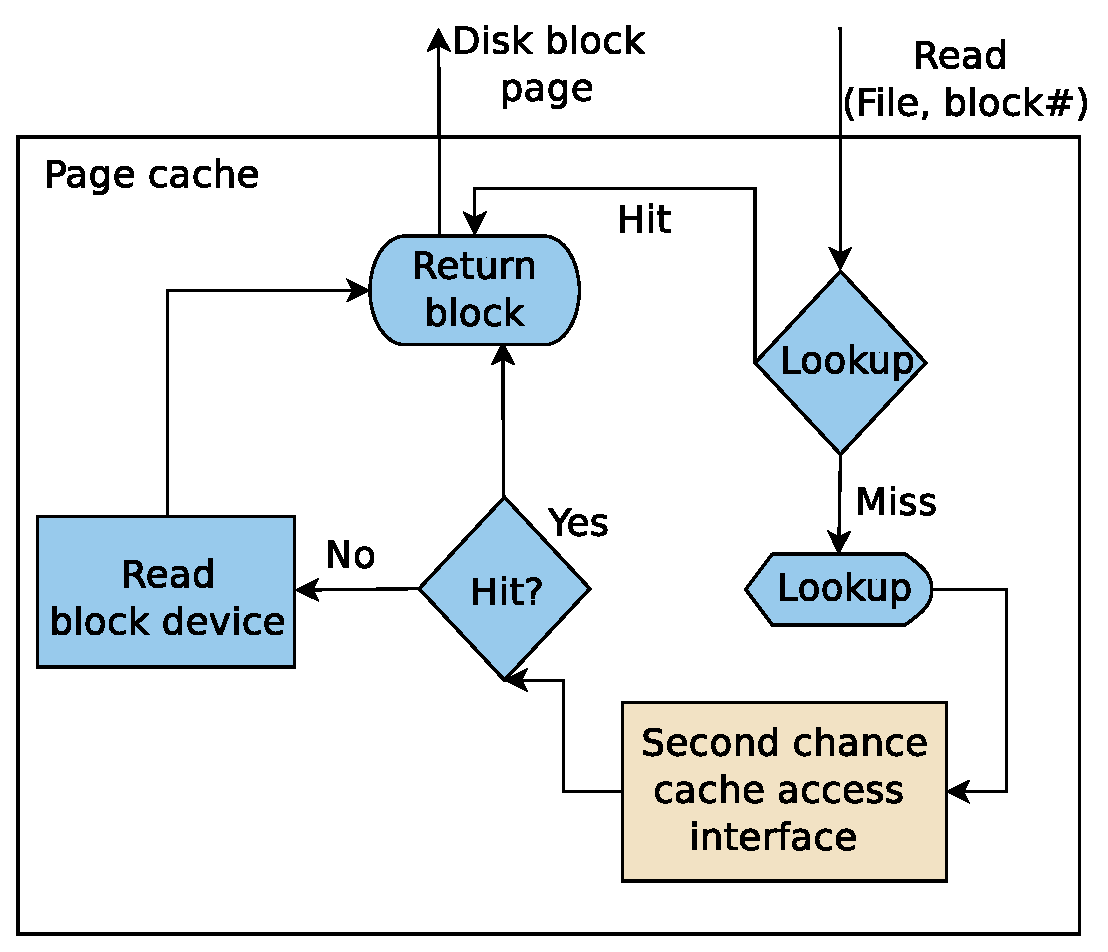
\includegraphics[width=\textwidth]{images/cc_get}
% \caption{Cache lookup of file block}
%\vspace{0.25cm}
% \label{fig:cc_get}
%\end{subfigure}

%\begin{subfigure}[b]{0.35\textwidth}
%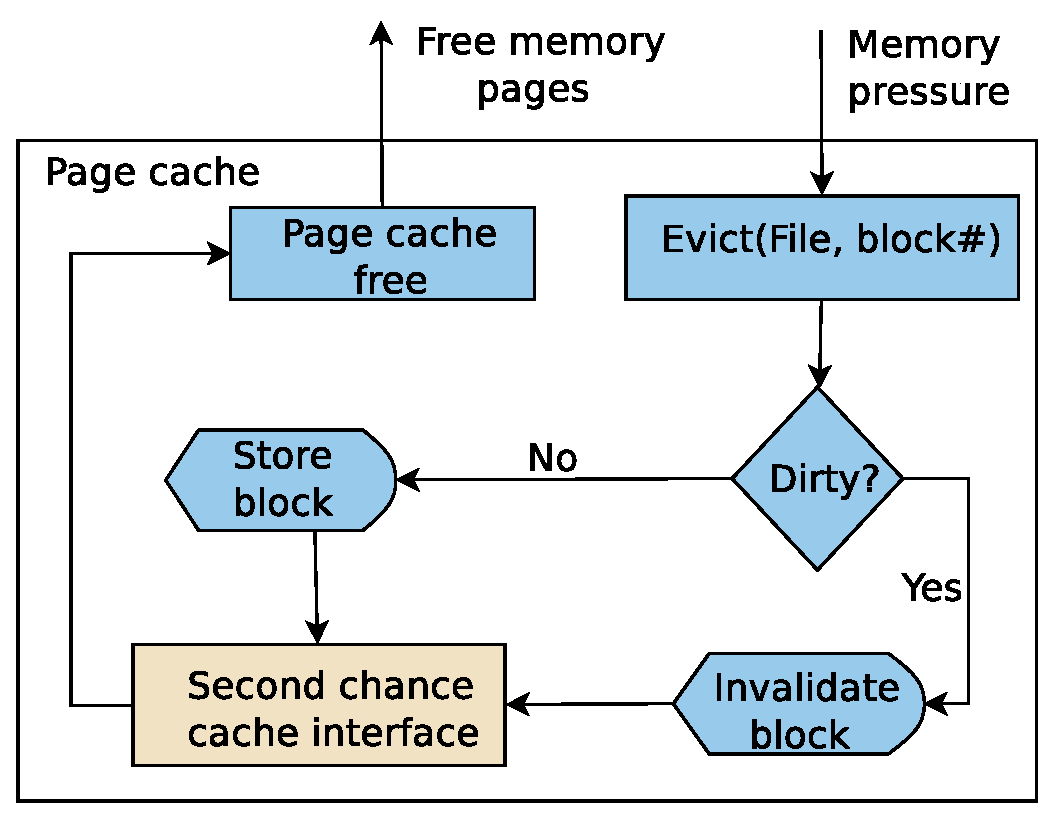
\includegraphics[width=\textwidth]{images/evict}
% \caption{Cache eviction of a file block}
% \label{fig:cc_evict}
%\end{subfigure}

%\caption{Operational view of second chance cache integration
%         with page cache.}
% \label{fig:cleanache_ops}
%\end{figure}

\subsection{Exclusive second chance caching}
\label{subsec:hcache}

\begin{figure}[t]
\centering
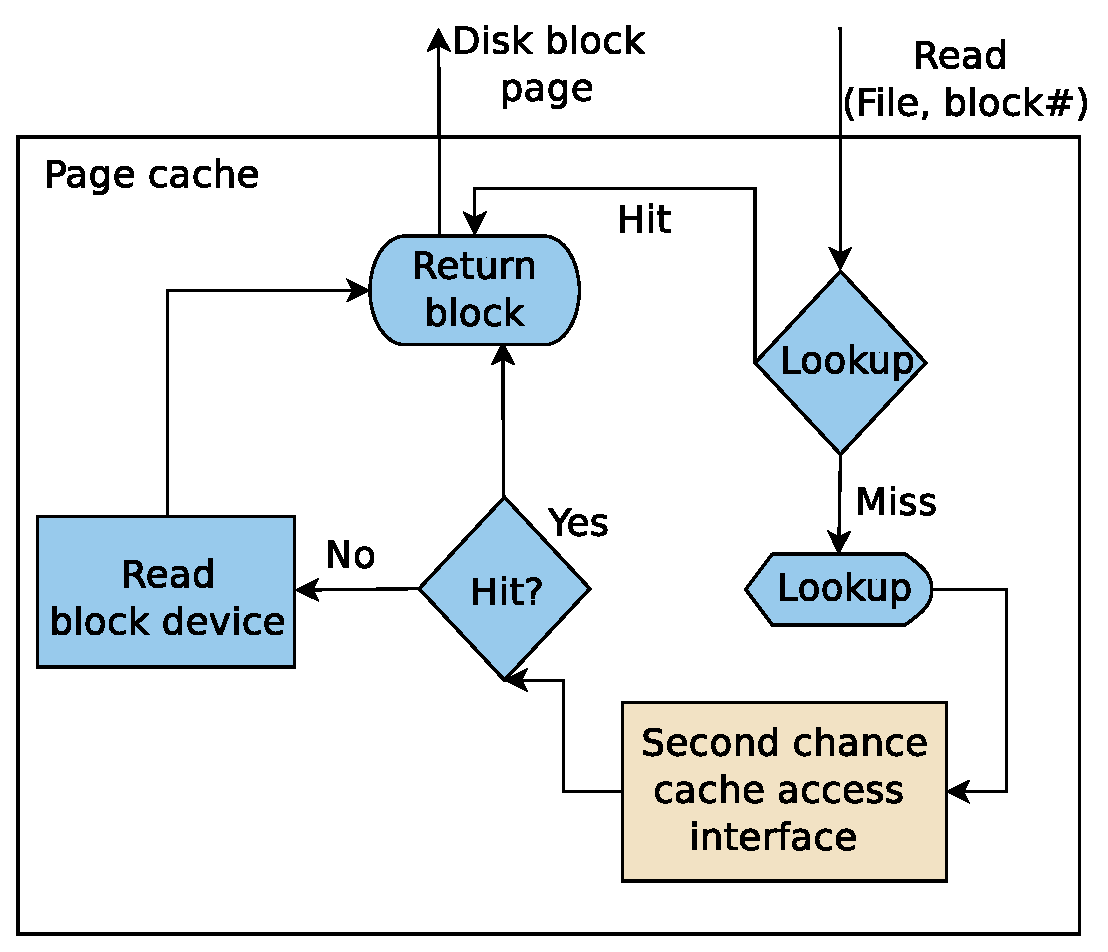
\includegraphics[width=0.35\textwidth]{images/cc_get}
 \caption{Cache lookup of file blocks in the page cache-second chance
cache integrated caching systems.}
 \label{fig:cc_get}
\vspace{-0.4cm}
\end{figure}


%
%\puru{Three figures is a too much for a subsection of the background.
%2a is the one to keep. Also 2a needs updates.}

%In Figure~\ref{fig:scache}, architecture of exclusive second chance cache
%is shown.
%%
%User space application initiated file IO requests are first looked up in the 
%operating system page cache to serve the requests without performing disk IO.
%%
With an exclusive second chance cache, application initiated file IO
requests are looked up in the OS managed disk page cache.
%
On a page cache miss, requests
are queried (lookup operation) in the second-chance cache (Figure~\ref{fig:cc_get}).
%
The second chance cache interface is tightly integrated with the page cache layer
and extends the IO path.
%to perform disk block lookup in the second chance cache in case of a page cache
%lookup failure.
%
When a clean disk block is evicted from page cache, a store operation is
initiated through the second chance cache interface.
%
To maintain exclusivity between the two caches, a block evicted from the
page cache is stored into the second chance cache and a block read from 
the second chance cache is removed from the second chance cache
and transferred to the page cache.

%
A generic second chance cache interface is implemented through 
%an actual 
%cache store implementation (Figure~\ref{fig:scache}) with choice of storage 
a cache store implementation using a storage option
(e.g., memory or SSD), storage optimizations (e.g., compression, deduplication) 
and, cache management policies for eviction and cache partitioning.
%
Linux \cleancache~\cite{cleancache}, an abstract second chance cache 
access interface, provides a generic second chance cache integration 
framework with the page cache.
%
The key operations of the interface are:---lookup (\get)
a disk block, store (\put)  a block in the cache and \flush{}
to invalidate objects from the cache (refer to Figure~\ref{fig:scache}).
%
In a virtualized setup, where second chance cache is implemented in the hypervisor, 
above operations ensure exclusive caching between the guest disk cache and
the hypervisor cache.
%
Hypervisor managed caches interface with the guest OS second chance
cache interface using
%hypervisor interfaces like hypercall (VMCALL)
the hypercall (VMCALL) API (Figure~\ref{fig:scache}).
%
The second chance stores only clean pages evicted from the page cache
and is indexed based on file system mount points or virtual machine
identifiers, the file information and the block number.
%
Several second chance cache implementations for native Linux and for
different virtualization solutions 
exist~\cite{zcache, oracletmem,kvmzcache, mortar}.
%
However, no state-of-the-art solution
supports application cognizant second chance cache management,
especially for nested hosting setups.
\begin{figure}[t]
  \centering
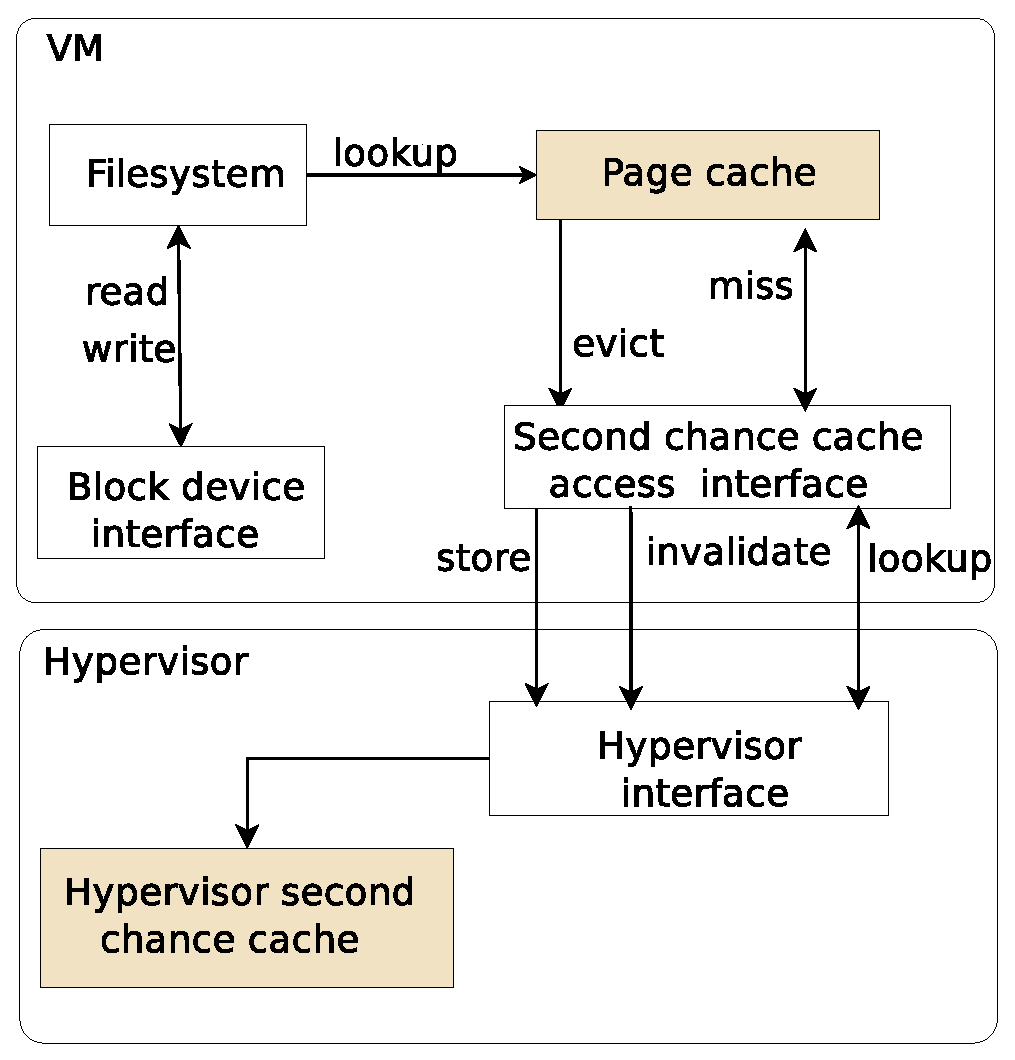
\includegraphics[width=0.35\textwidth]{images/tmem}
 \caption{Overview of second chance cache integration with OS page cache 
with exclusive mode of operation.}
 \label{fig:scache}
\vspace{-0.2cm}
\end{figure}
%can be part of the operating system (e.g., \zcache{} in
%the Linux OS~\cite{zcache}) or part of the hypervisor in a virtualized 
%system~\cite{oracletmem,kvmzcache,mortar}. 
%
%
%The block device interface is used as the last resort to access blocks from the disk
%on cache lookup failure at both the page cache and the second chance cache.
%
%\subsubsection{Exclusive second chance cache operations}
%\label{subsec:hcache}

%Transcendent memory (or \tmem{})~\cite{oracletmem} is a state-of-the-art
%hypervisor-managed cache which implements exclusive caching by
%design~\cite{memtrans}.
%
%The \tmem{} cache stores \emph{clean} disk pages
%does not contain dirty data at any
%point in time 
%and thus is transparent to storage durability mechanisms.
%
%An example hypervisor caching framework (illustrated in Figure~\ref{fig:tmem}) 
%has three major components---(i) a guest OS \cleancache{} interface, (ii) a hypervisor 
%managed back-end cache, and (iii) a hypervisor interface to access the cache.
%
%On a disk page lookup failure in the first chance cache (page cache),
%second chance cache  lookup (a \get{} operation) is performed 
%to {\em find-and-fetch} the requested block from the second chance cache 
%onto the page cache as shown in Figure~\ref{fig:cc_get}.
%%
%If the block is not found in the second chance cache, a block IO request is
%initiated to fetch the block from the block device.
%
%Similarly, when the page cache layer is requested to evict clean/unmodified cached 
%disk blocks, the block is stored in the second chance cache (a.k.a \put{} operation)
%(Figure~\ref{fig:cc_evict}). 
%%
%%For a dirty block eviction, second chance cache invalidate (\flush) operation
%purges the page from the second chance cache, if present, since the second chance
%cache version of the page is now outdated.
%
%

%The unique key provided by the \cleancache{} abstract interface is a three 
%tuple i.e., file system mount point ID (\texttt{pool-id}), 
%file identifier (\texttt{inode number}) and the block offset of the requested 
%file block.
%%cache provides a key-value interface for storing page
%%objects.
%%
%The second chance cache store is responsible for mapping these keys to actual
%storage objects to implement \get, \put{} and \flush{} operations.
%%
%%The \texttt{pool-id} is negotiated during the file system initialization. 
%
%In a hypervisor cache implementation, the hypervisor cache is additionally responsible
%to uniquely identify requests from different VMs which is typically ensured by extending the 
%key with an additional \texttt{vm-id} element.

\subsection{Application container isolation framework}
%
Light-weight resource isolation frameworks like Linux control 
groups (\cgroup)~\cite{cgroup} provide performance isolation 
across multiple execution domains with low virtualization 
and multiplexing overheads compared to hypervisor enabled 
system virtualization solutions.
%machine level isolation solutions.
%
Linux \cgroup~\cite{cgroup} and FreeBSD Jails~\cite{jail} are examples
of performance isolation frameworks facilitating resource management 
for a group of processes by specifying group-level resource limits.
%for different
%resources e.g., CPU time, memory size, network and disk bandwidth etc..
%
%For example, to manage memory across \cgroups, two control knobs 
%i.e., \texttt{hard limit} and \texttt{soft limit} are provided in Linux \cgroup{}
%resource control model.
%
Using the process grouping based isolation model, container management
solutions like LXC~\cite{lxc} and Docker~\cite{docker} enable hosting
multiple applications in different application groups (containers).
%

%In a nested hosting system like derivative clouds, the two resource control 
With containers in virtual machines derivative clouds, 
the two resource controllers---the hypervisor and the \cgroup{} subsystem---operate 
in an agnostic manner w.r.t. each other.
%
As a result, centralized/global hypervisor cache 
distribution from the containers perspective is not 
deterministic (\S\ref{subsec:motivation}).
%is uncontrolled and arbitrary (\S\ref{subsec:motivation}).
%
To enable differentiated partitioning of the hypervisor cache and 
to facilitate intelligent use of multiple storage backends across 
containers, it is necessary to design a
solution that can provide synergy across the two control points.
%

\subsection{Motivation}
\label{subsec:motivation}
%\begin{figure*}
%\centering
%\begin{subfigure}{0.5\columnwidth} 
%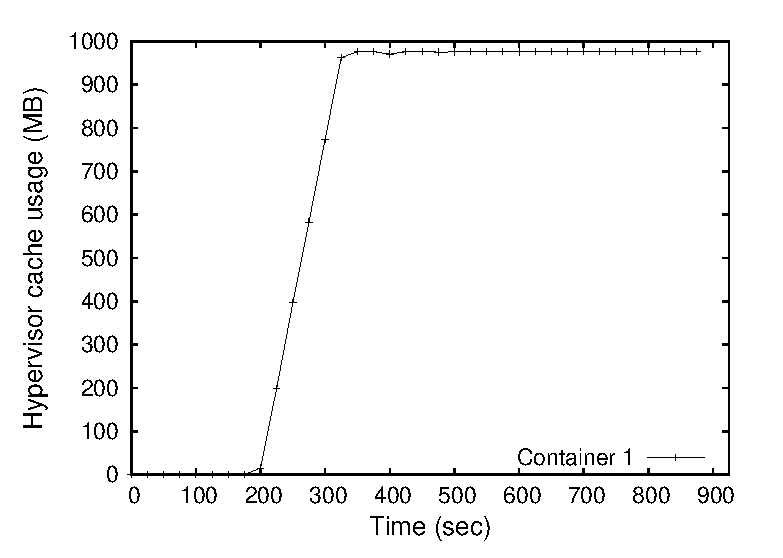
\includegraphics[width=\columnwidth]{data/motivation/disparity_c1} 
% \caption{Application container 1}
% \label{fig:cachedistrib1} 
%\end{subfigure} \hfill
%
%\begin{subfigure}{0.5\columnwidth}
%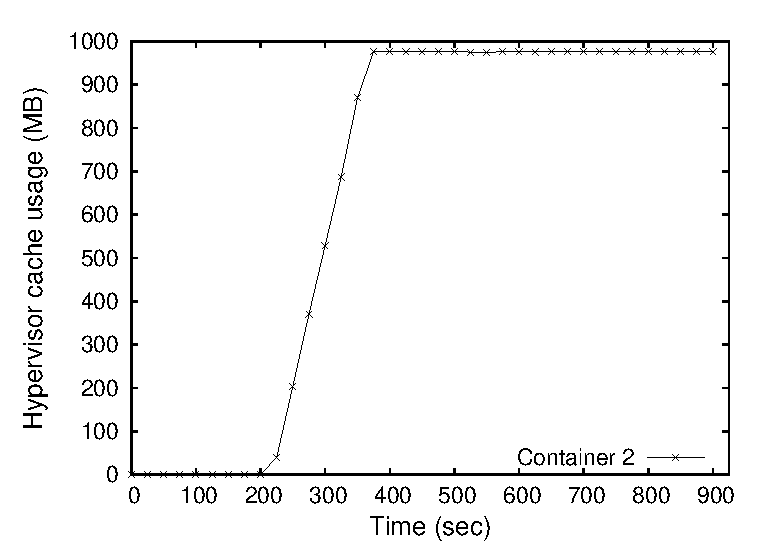
\includegraphics[width=\columnwidth]{data/motivation/disparity_c2} 
% \caption{Application container 2}
% \label{fig:cachedistrib2} 
%\end{subfigure} \hfill
%
%\begin{subfigure}{0.5\columnwidth}
%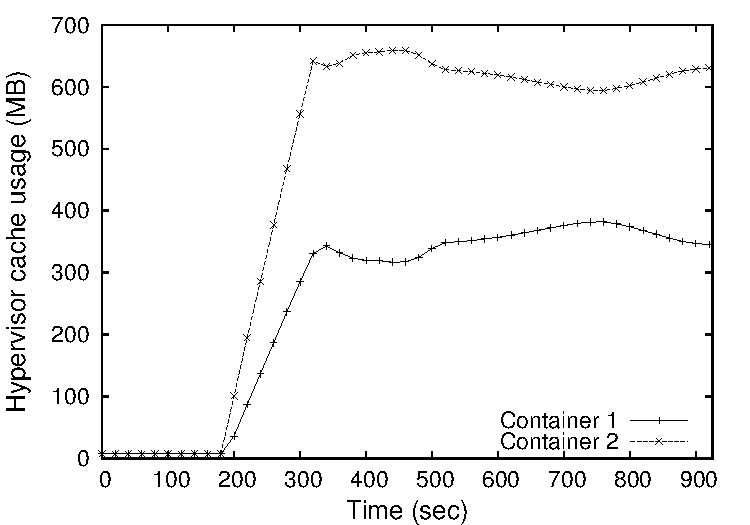
\includegraphics[width=\columnwidth]{data/motivation/disparity1}
% \caption{Application containers 1 and 2}
% \label{fig:cachedistrib12} 
%\end{subfigure} \hfill
%
%\begin{subfigure}{0.5\columnwidth}
%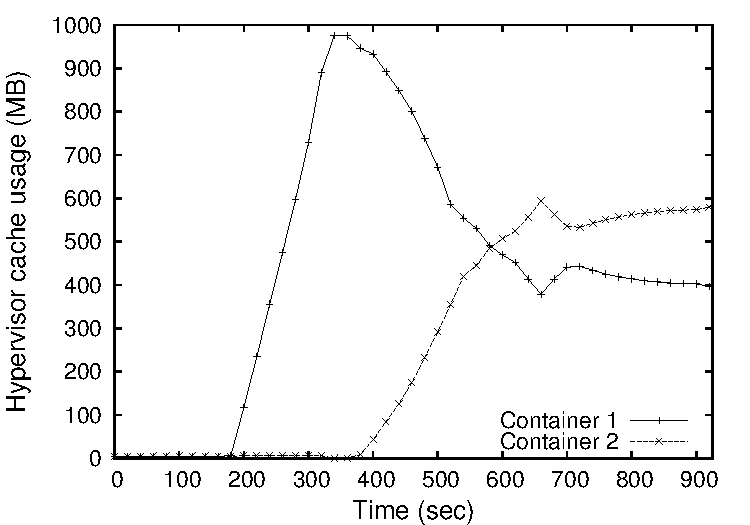
\includegraphics[width=\columnwidth]{data/motivation/disparity2}
% \caption{Application containers 1 and 2}
% \label{fig:cachedistrib12_offset} 
%\end{subfigure} \hfill
%
%\caption{Hypervisor cache distribution across two containers hosted inside a VM.}
%\label{fig:cachedistrib}
%\end{figure*}
\begin{figure}
\centering
\begin{subfigure}{0.49\columnwidth} 
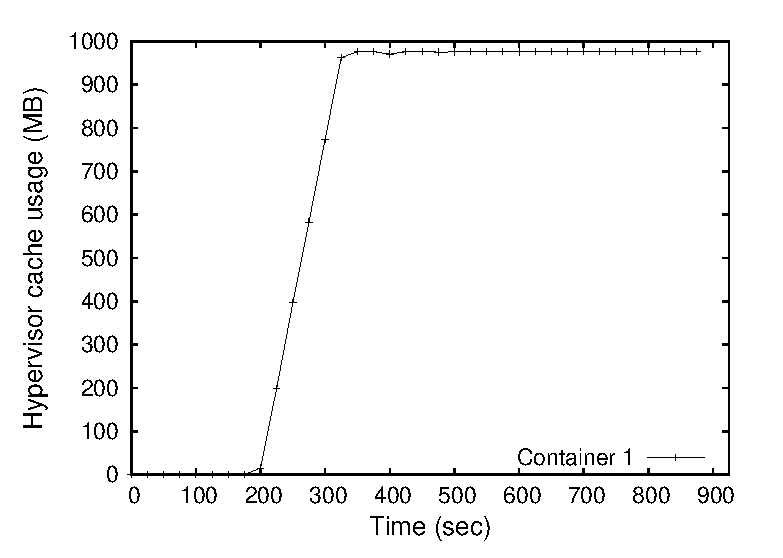
\includegraphics[width=\columnwidth]{data/motivation/disparity_c1} 
 \caption{Application container 1}
 \label{fig:cachedistrib1} 
\end{subfigure} \hfill
%
\begin{subfigure}{0.49\columnwidth}
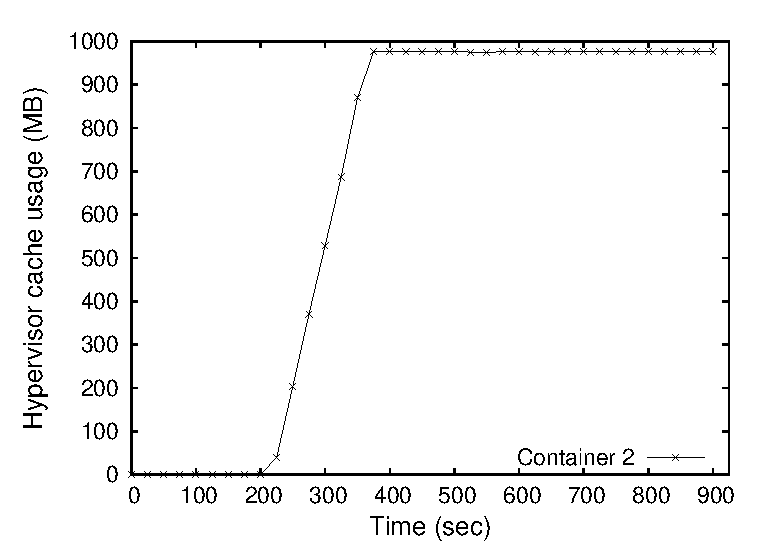
\includegraphics[width=\columnwidth]{data/motivation/disparity_c2} 
 \caption{Application container 2}
 \label{fig:cachedistrib2} 
\end{subfigure} \hfill
%
\caption{Hypervisor cache distribution when application containers
         executed separately.}
\vspace{-0.3cm}
\label{fig:separate}
\end{figure}


\begin{figure}
\centering
\begin{subfigure}{0.49\columnwidth}
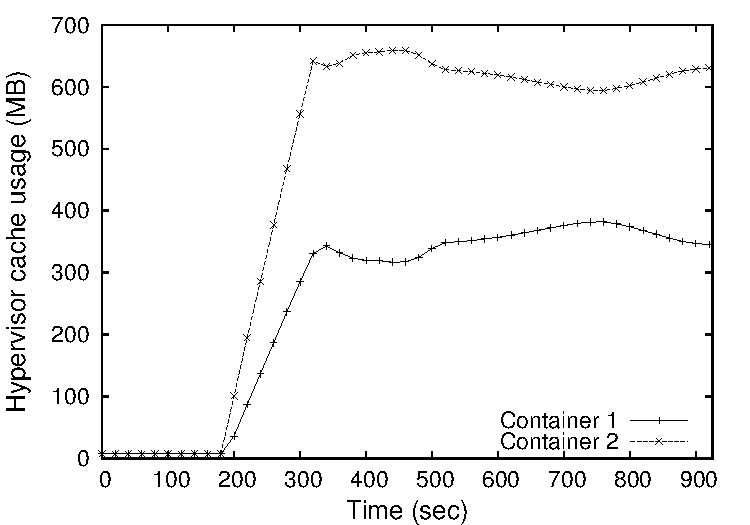
\includegraphics[width=\columnwidth]{data/motivation/disparity1}
 \caption{Same start time}
 \label{fig:cachedistrib12} 
\end{subfigure} \hfill
%
\begin{subfigure}{0.49\columnwidth}
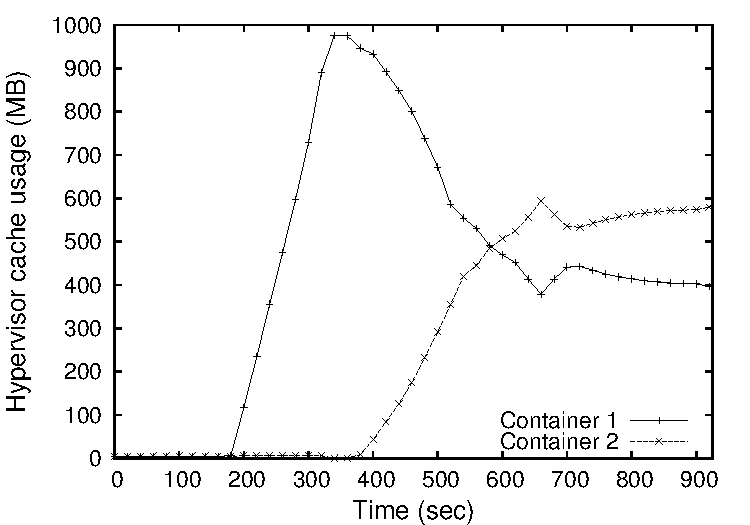
\includegraphics[width=\columnwidth]{data/motivation/disparity2}
 \caption{Container 2 offset by 200 sec}
 \label{fig:cachedistrib12_offset} 
\end{subfigure} \hfill
%
%\caption{Hypervisor cache distribution when application containers
%         executed simultaneous with different application start times.}
\caption{Hypervisor cache distribution with different start times of
application containers.}
\vspace{-0.4cm}
\label{fig:together}
\end{figure}


To demonstrate the non-deterministic cache distribution in a nested 
container setup, we performed an experiment with a VM configured 
with 2GB memory and 4 VCPUs on a host with 32GB memory and 16 CPUs.
%
The hypervisor cache 
was not cognizant of the containers and its size was limited to 1GB.
%was similar to Xen tmem~\cite{oracletmem} which
% i.e., cache limit enforcement was on a per-VM basis.
%
%The maximum hypervisor cache limit was set to 1GB for this experiment.
%
Two application containers (Container 1 and Container 2) configured with 
the same memory limits (through \cgroup) executed the \web-workload of the 
\file~workload suite~\cite{filebench}.
%
The only difference between the two containers was their IO load; 
Container 1 executed two
\web~threads while Container 2 executed three \web-threads.
%

With this setup, when Container 1 and Container 2 executed separately one-at-a-time, 
each of them used up the entire hypervisor cache (Figure~\ref{fig:separate}).
%as shown in 
%Figure~\ref{fig:cachedistrib1} and Figure~\ref{fig:cachedistrib2}, respectively.
%
The implication being that each application is capable of taking advantage 
of the configured hypervisor cache to its capacity when executed separately.
%
%To show the non-deterministic cache distribution behavior, we performed an 
%experiment with the same setup where both application containers shared the 
%hypervisor cache during
%the workload execution.
%

When both applications were started simultaneously,
the hypervisor
cache was distributed across containers in a disproportionate manner.
%
Share of Container 2 was approximately two times that of
Container 1 as shown in Figure~\ref{fig:cachedistrib12}.
%
The non-determinism is a side-effect of the IO load and
the FIFO-based global eviction policy (not ensuring container level fairness) 
of the hypervisor cache.
%
%In another hypervisor cache sharing experiment (Figure~\ref{fig:cachedistrib12_offset}),
When Container 2 started executing its  workload after a delay of 200 seconds 
form start of workload in Container 1,
%that of container 1 application start time.  
%
%In this case, container 1 dominated the cache usage in initial part, after which
Container 1 dominated the cache usage till about 500 seconds, after which
cache share of Container 2 increased before surpassing that of 
Container 1 at around 600 seconds(Figure~\ref{fig:cachedistrib12_offset}).
%
%\puru{maybe we should add a table to compare performance with
%deterministic cache sizing.}
%These results demonstrate the non-determinism in cache distribution across 
%application containers executing inside the VMs
%, specifically in case of derivative 
%cloud setups.
%
%Therefore, 
These results demonstrate that state-of-the-art hypervisor caches are unable to
implement policies (e.g., fair allocation to application containers) in a 
deterministic manner at a sub-VM granularity.
%

\subsubsection{VM level memory management flexibility}
\label{subsec:sdc}
%
%
\begin{figure}[t]
  \centering
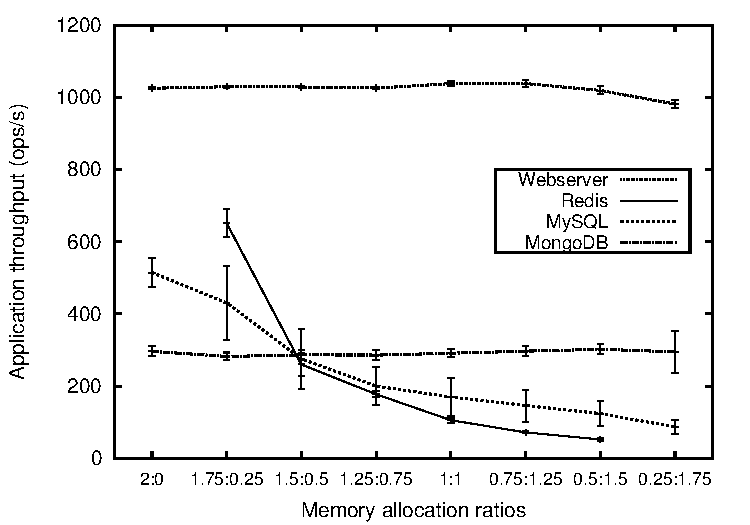
\includegraphics[width=0.45\textwidth]{images/appl_behavior} 
 \caption{Application performance with different provisioning configurations 
  at the two levels of a derivative cloud.}
 \label{fig:app_behavior} 
\end{figure}
%
To analyze the impact of memory provisioning at the two 
levels (guest OS and hypervisor cache) in a nested setup and motivate the need for 
guest OS control on the hypervisor cache sizing, we performed the 
following experiment.
%
2GB memory was split in different ratios to allocate memory for the container 
inside the VM (through Cgroups) and the hypervisor cache.
%
For example, an allocation ratio of 1.5:0.5 (Figure~\ref{fig:app_behavior}) refers to
a 1.5 GB in-VM memory limit and 0.5 GB hypervisor cache limit for
the container. 
%
Application performance for four different workloads,
the Filebench \web{} workload and YCSB~\cite{ycsb} using 
Redis, MongoDB and MySQL data stores,
with different allocation ratios is shown in 
Figure~\ref{fig:app_behavior}. 
%
Application throughput for Webserver and MongoDB remain almost unchanged 
(1000 ops/sec and ~300 ops/sec, respectively) while Redis and MySQL performance 
degraded when more memory was split with the hypervisor cache.
%
Redis was exceptional in extreme split scenarios---very high throughput (10406 ops/sec) was
observed with 2GB VM memory allocated to the container and, application stall observed when 256 MB 
memory was allocated through the Cgroup and rest allocated in the hypervisor cache.
%
\begin{table}[t]
%\scriptsize
\begin{center}
\begin{tabular}{|c|c|c|c|}
\hline
{\bf Application} & {\bf Total} & {\bf Anonymous} & {\bf Hypervisor} \\
{\bf usage } & {\bf swap} & {\bf memory} & {\bf cache} \\
 & {\bf (MB)} & {\bf usage (MB)} & {\bf usage (MB)} \\
\hline 
\hline 
Websever & 0 & 88.9 & 1023 \\
Redis & 996 &  1021 & 18.5 \\
MySQL & 879 & 1013 & 34 \\
MongoDB & 0 & 251 & 1023 \\
\hline 
\end{tabular}
\caption{Guest OS metrics for different applications with equal split (1GB in-VM and 1GB 
         hypervisor cache) scenario.}
\label{table:app_diagnosis}
\vspace{-1cm}
\end{center}
\end{table}

Explanation for the application behavior is presented in 
Table~\ref{table:app_diagnosis}.
%
Applications requiring anonymous memory can not be helped by the 
hypervisor cache and resort back to swapping as the last alternate.
%
For applications depending on file I/O, hypervisor cache 
can offload the caching responsibility without causing any
application degradation.
%
These results show that providing the VM level memory manager with the option
to choose different cache and in-VM memory configurations provides flexibility
to meet various application SLA objectives.

 
%
%Hypervisor caching solutions with application level differentiated 
%management fall short to facilitate decentralized policy enforcement.
Existing centralized hypervisor cache management 
techniques (e.g., Morai~\cite{sdc}, Centaur~\cite{centaur}) have
limitations w.r.t. their applicability in such scenarios.
%
The required flexibility to empower VM-level memory management across
applications (as deduced from the previous experiment) is not supported.
%
For example, existing techniques can neither improve performance of the 
applications that depend on anonymous memory allocations (e.g., Redis) 
nor provide flexibility to free in-VM memory by selectively offloading 
applications (e.g., Webserver) to the hypervisor cache.
%
%Some additional drawbacks in the existing hypervisor caching 
%solutions are mentioned below. 
Additionally, existing hypervisor caching solutions~\cite{sdc,centaur}
%
%First, they operate in an inclusive cache operation mode
operate in an inclusive cache operation mode
w.r.t. the guest OS page cache which is wasteful due to duplicate 
storage of disk blocks in memory.
%
%Second, 
Further, application differentiation at the hypervisor cache is not
generic. For example, Morai~\cite{sdc} requires applications to be 
hosted on different virtual disks so that they can be distinguished at the
hypervisor level.
%


%
To support differentiated policy enforcement in derivative cloud setups
at the nested levels, a rethink of the hypervisor cache design is required.    
%
The proposed design should allow independent memory management at the two 
nested levels with the hypervisor still being the enforcing entity. 
%

%\section{Architecture and Design}
\section{\dd{} Architecture}
\label{sec:design}

\begin{figure}[t]
  \centering
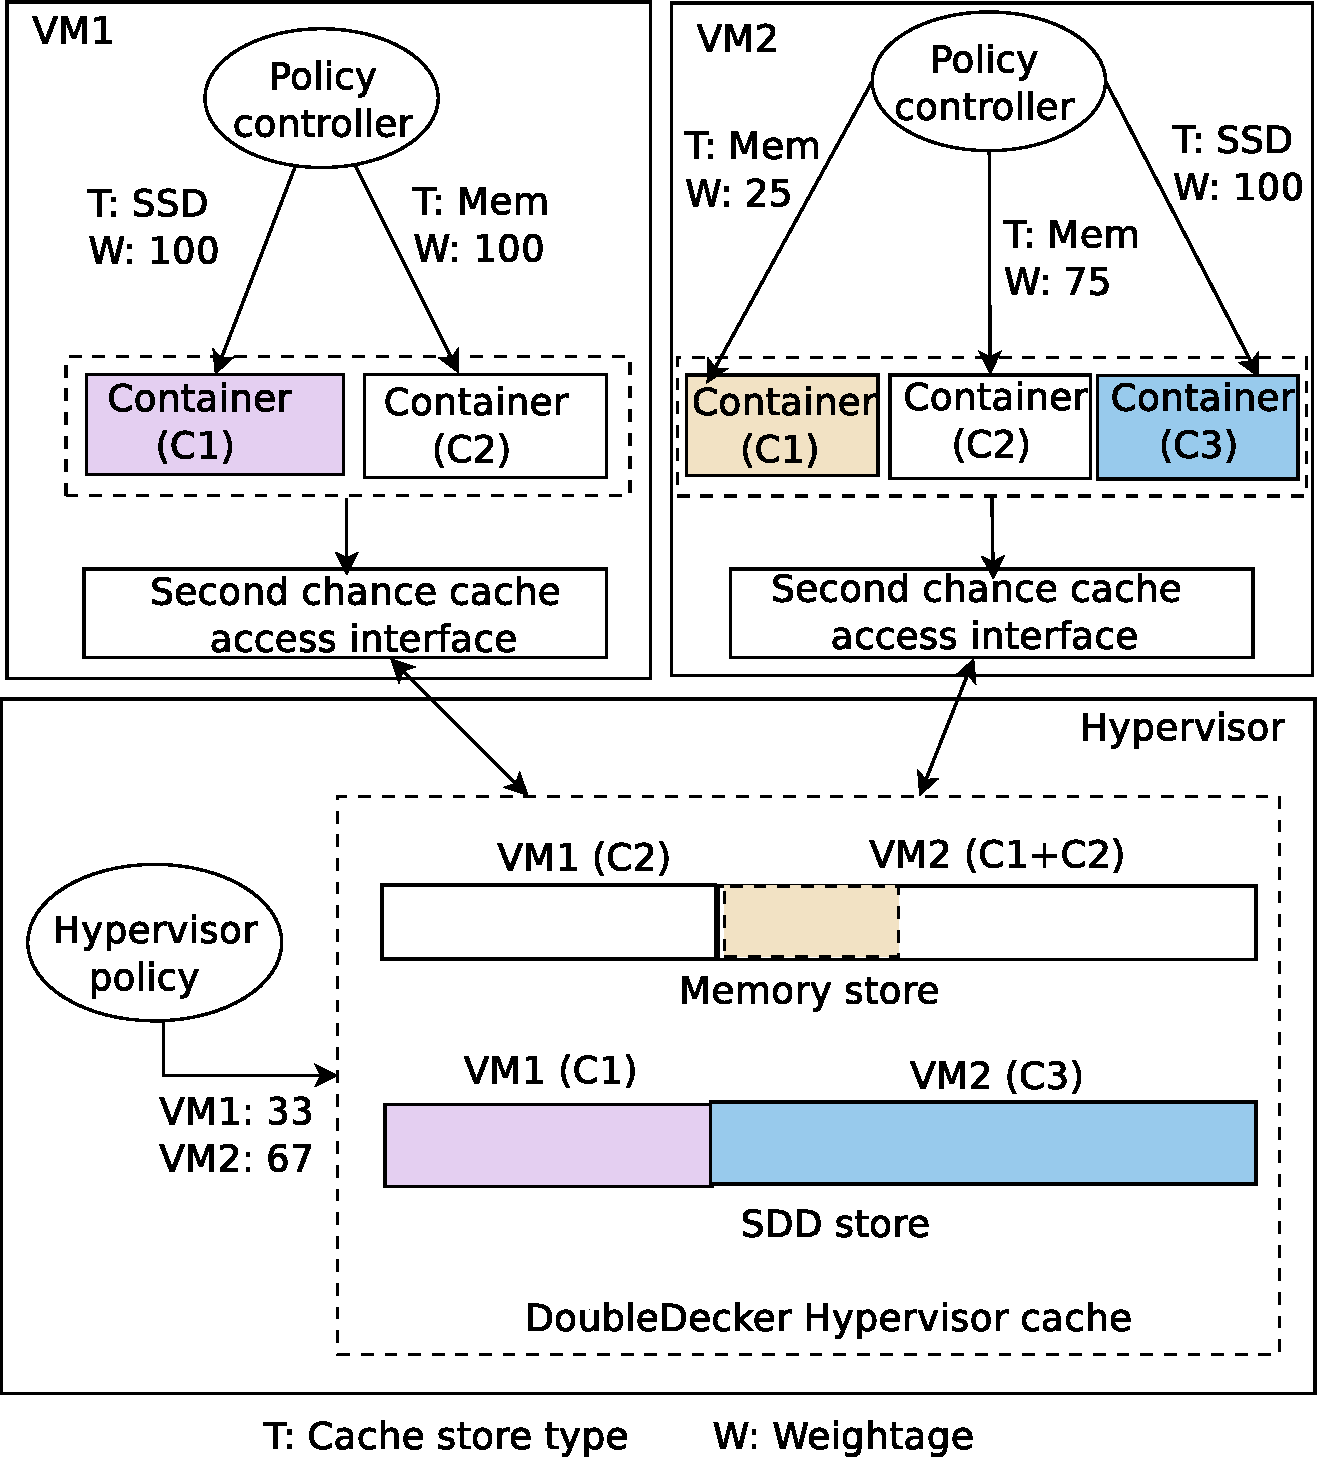
\includegraphics[width=0.42\textwidth]{images/arch} 
 \caption{Proposed differentiated hypervisor cache partitioning 
          across containers in a nested virtualization setting.
	 % \puru{figure needs updates. 1:2 vs. 25:75:100 ... consistently
	 % lets use ratios or weights. Should also probably include a ddecker
	 % cache manager in the hypervisor.}
         }
 \label{fig:desired} 
\vspace{-0.3cm}
\end{figure}

\dd{} provides a 
multi-layered differentiated cache partitioning and management solution.
%\dd{} solution framework for container aware hypervisor caching
%with multi-layered differentiated cache partitioning and management
%is presented in Figure~\ref{fig:desired}.
%
The software architecture of \dd{} is as shown in Figure~\ref{fig:desired}.
Its two main components are the second chance cache interface housed
in each virtual machine and the \dd{} cache manager augmenting the 
hypervisor.
%
The hypervisor cache is managed via two policy controllers,
one to control per-VM provisioning and the other
to control per-container provisioning in the corresponding
virtual machines cache region.
%
Our current design specifies allocations in terms of cache 
usage \revised{weights} in percentage between peer entities at 
each hosting level. 
%
Additionally, the policy controller in each virtual machine
also specifies the cache store type of each container.
%
A two tuple \texttt{<T, W>} is used for this purpose,
where, \texttt{T} denotes the store type (in-memory or SSD)
and \texttt{W} the weight specification for relative sizing.
%
%To configure and manage hypervisor cache, two policy control interfaces provided in 
%the proposed design---(i) VM level policy configuration by the hypervisor, (ii) Container
%level policy specification by the VM administrator. 
%
%The VM level policy is specified in relative weights of the VMs using which
%the hypervisor cache is partitioned across the VMs.  
%%
%Container level policy is specified by a two tuple for each VM---(i) T: cache store type,
%(ii) W: cache usage percentage.
%%
%Cache store type (T) in the proposed architecture is to provide support for multiple types of
%cache stores which can be queried from the VMs and every container can be configured
%with storage backend type as dictated by the policy.
%

Figure~\ref{fig:desired} shows a setup with two virtual machines
with a cache allocation \revised{weight} percentage of 33 and 67. 
The per-VM ratio is
applied to both the memory and the SSD store across all VMs
\footnote{A generalized setup where different cache size
ratios are specified per-VM for the two stores is a straightforward
extension.}.
%
The first virtual machine, VM1 hosts two containers and the second VM (VM2)
hosts three containers.
%In the example setup shown in Figure~\ref{fig:desired}, 
%there are two VMs---VM1 and VM2---configured with weightage
%ratio of 1:2 by the hypervisor.
%
%Two and three application containers are instantiated in VM1 and VM2%,
%respectively.
%
%Each VM administrator can use the policy interface to
%specify the weights for each container's hypervisor cache share.
%
Virtual machine administrators use the local policy controller
to specify distribution of the per-VM cache space across containers.
%
For the example shown, the specification for VM1 for its two
containers is $<$SSD, 100$>$ and $<$Mem, 100$>$---Container 1 to be allotted
all of VM1's share in the SSD store of the hypervisor cache and Container 2
to be allotted all of VM1's share in the memory store of the cache.
%
Similarly, the specification for VM2 is to allocate its memory
store in the ratio of 1:3 for the first two containers and allocate
all of its share in the SSD store to the third container.
%
%In this case, Container 1 and Container 2 of VM1 are configured to use the 
%VM's share of SSD and memory backed cache store, respectively.
%
%
%Container 1 and Container 2 of VM2 are configured with memory backed 
%hypervisor cache with usage percentages as 25 and 75, respectively. 
%
%Container 3 of VM2 is configured to used SSD backed cache store.
%
Based on the above specifications the hypervisor memory store
is shared by three containers and the SSD store by two.
%
Simultaneously, the \revised{weights} for VM1 and VM2 for both the stores
are 33 and 67, respectively.
%
%As shown in the Figure~\ref{fig:desired}, hypervisor cache gets
%distributed depending on the configured weightages at two levels---between
%VMs and across containers within each VM.
%
%Hypervisor memory store is shared by three containers---Container 2 of VM1 and,
%Container 1 and Container 2 of VM2---in the proportions derived by first applying
%relative VM weightage and next by applying container share limits within each VM's
%share.  
%
%Similarly, SSD backed hypervisor cache is shared by Container 1 of VM1 and Container
%3 of VM2 in the ratio of the relative priorities of the VMs.
%
%Different components in the proposed design are explained further.
%\puru{add transition line here.}

\subsection{Policy control mechanism}
The \cgroup{} resource control framework for instantiating containers
provides configuration options to specify allocation limits 
for different resources, e.g.,
CPU share, memory usage limit etc. per-cgroup.
%
Additionally, for each container, the \dd{} policy controller requires 
specification of the hypervisor cache storage type and weight for cache sizing.
%
An extension to the \cgroup{} resource control framework is warranted to 
incorporate this feature.
%
Similar to the dynamic adjustment of resource limits, the hypervisor
cache specifications are required to be handled in dynamic manner.
%the additional configurability related to hypervisor caching.
%
%Container resource control through \cgroups{} should support dynamic
%specification of the policy and propagation of the same to the hypervisor 
%cache store.
%
Interfacing of the updated \cgroup{} resource control framework 
also requires extensions to the second chance cache access 
interface in the guest OS.
%with the hypervisor cache
%interface requires redesign of the hypervisor cache interface.

\subsection{Second chance cache access interface}
The second chance cache interface (explained in \S\ref{sec:bg}) 
assigns unique pool identifiers to each file system registered to use the 
second chance cache by delegating the call to the cache store
implementation.
%
The unique pool identifier is an integral part in the key 
used for operations like lookup, store etc..
%
%which is used for second chance cache operations
%like \get, \put{} and \flush. 
%
%In the proposed system, 
In a derivative cloud setup several containers can be instantiated 
within a single file system, making file system based identifiers 
not applicable.
%which implies file system IDs can not be used as an identification for 
%containers.
%
Towards addressing this, extensions to the \cgroups{} subsystem and 
the second chance cache interface need to be integrated so that 
an unique identity is assigned to each application container 
for use by the hypervisor cache.
%This fundamental change requires redesign of the interface in such 
%a manner that
%each application container uses an unique identity which is assigned 
%by the hypervisor cache store.
%
When an application container boots up, the hypervisor cache interface 
is notified by the \cgroups{} subsystem, which in turn
requests a new pool-ID from the hypervisor cache.
%and assigns the pool ID
%to the application container for its life time.
%
Subsequent second chance cache accesses 
issued by the guest OS are accompanied by the container specific
unique pool identifier.
%because of page cache
%look up failures or evictions 
%
The unique pool-ID is derived by determining the container for the 
operation.
%
%For example, a second chance lookup (\get) request for a file block is first mapped
%to the application container responsible for this lookup to derive the pool ID and pass it 
%on to the hypervisor cache store.
%
%
\subsection{Hypervisor cache store}
%
The cache store implementation of \dd{} %hypervisor cache store 
is required to support container-level policies apart from 
providing VM-level cache partitioning. 
%
The VM-level cache partition sizes are derived from 
ratios specified via the hypervisor-level policy controller.
%\puru{administrator vs. hypervisor level policy.}
%administrator configured ratios 
%
To apply application container level policies, configurations for
containers are transmitted to the hypervisor cache manager
via the guest OS cache interface.
%delegated to the hypervisor cache.
%
%As mentioned earlier, every application container is assigned an unique
%pool ID on start up.
%
The hypervisor cache store applies the policies to partition the
cache across the containers of a virtual machine and also maintains
cache proportionality across virtual machine.
%
The \dd{} solution provides backend storage implementation with
support for dynamic reconfiguration of policies, both at the
hypervisor-level and from within virtual machines. 
%
This feature is required
for dynamic provisioning with changing workload characteristics of
applications and to handle instantiation and removal of virtual
machines and containers.
%
With the derivative setup, a virtual machine can choose to store
objects of all its containers in memory, or on the SSD or 
distributed over both in-memory and SSD storage 
%split storage destinations 
on a per-container basis.
%

\revised{The hypervisor cache also implements an eviction procedure
to flush objects in the cache during memory pressure.
%
%As part of this work, we implement a FIFO policy for
%evictions of objects on memory pressure.
%
}
With two types of storage options available,
a \emph{trickle-down} and \emph{trickle-up} cache is possible---
objects evicted from the second-chance cache are stored
in the third-chance cache.
%
The design of \dd{} is centered around the idea that the
semantics and decisions of how to manage the hypervisor cache
should be left to the policy controller in the guest
operating systems.
%
This offers flexibility to the policy engine to explicitly 
size and choose the storage type for individual applications.
%
For example, a policy engine can decide that an application
that does mostly sequential reads or one whose working set
size is very large, should have its objects stored in 
the SSD.
%
%Storing such objects and then ``spilling'' them over the
%third-chance cache will only pollute the second-chance
%cache.
%
%We present empirical results to demonstrate this in Section~\ref{sec:expt}.
Nevertheless, keeping the core principle of supporting cache management from 
within the VM, we provide a hybrid mode configuration option for the
VM-level controller.
%
In this mode, the VM-level controller can provision containers 
with both memory and SSD shares, where the SSD store is used only when the
memory share of the container is exhausted. 
%
The comprehensive design and evaluation of the hybrid store
is left as a future direction. 
%
In this work, we present
results with applications configured to use either in-memory
or SSD backed caches, not both.
%
%
%memory and SSD.
%
%Depending on memory type configuration for the containers, the requests
%are stored either in the memory store or the SSD store.
%

\revised{
While exclusive caching takes care of deduplication of memory across 
the hypervisor cache and page cache of individual virtual machines, there is 
a chance of content duplication across virtual machines and the hypervisor
cache.
%
Holistic deduplication techniques in virtualized systems~\cite{synergy} can be 
incorporated into DoubleDecker to address the issue of duplication and left as
a future direction. 
}

\section{Implementation}
\label{sec:impl}
\begin{figure}[t]
  \centering
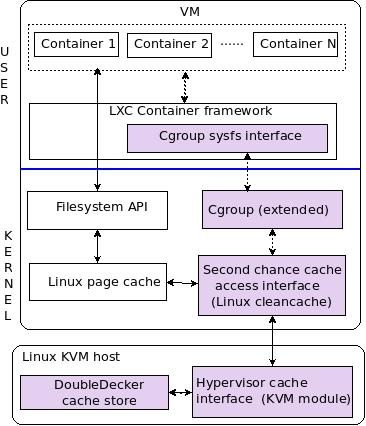
\includegraphics[width=0.4\textwidth]{images/implementation} 
 \caption{\dd{} implementation in KVM virtualized system. The shaded 
 boxes in the figure represents modified/enhanced software components.
% \puru{this figure not refered in text?}
}%
 \vspace{-0.5cm}
 \label{fig:impl} 
\end{figure}

We implemented the \dd{} solution on the Linux+KVM virtualization
platform and LXC~\cite{lxc} containers.
%We have implemented \dd{} in Linux KVM hypervisor platform.
%
Guest OS modifications are implemented in Linux virtual machines
hosting LXC~\cite{lxc} containers.
%
Linux \texttt{cleancache}, the second chance cache access interface 
is modified to implement the \cgroup{} extensions required for \dd{} (Figure~\ref{fig:impl}).
%hypervisor cache store.
%
Linux \cleancache{} operations are routed to the KVM hypervisor through 
a new VMCALL~\cite{intelmanual}.
%
As shown in Figure~\ref{fig:impl}, the KVM hypervisor module is 
modified to capture this hypercall, 
copy the arguments on to the host memory and pass the call to 
the \dd{} hypervisor cache store. 
 

\subsection{\cgroup{} and \cleancache{} modifications}
%
Several modifications to the Linux \cgroups{} subsystem
are required for container-level nested hypervisor cache management.
%
Two new parameters have been added to the kernel
state description of the \cgroups{} subsystem---
(i) name of the \cgroups{} for
which the hypervisor cache is to be enabled, 
(ii) policy configuration tuple ($<$\texttt{T, W}$>$) for each container 
to specify 
the storage type and weightage percentage.
%\puru{what is identification filter?.}
%
These parameters can be accessed as \texttt{sysfs} entries 
from the user space.
%user space 
%(sysfs) configurations---(i) name or identification filter of the \cgroups{} for
%which the hypervisor cache is to be enabled, (ii) policy configuration tuple
%for each container to specify the storage type and weightage percentage.
%
Interactions between the \cgroup{} subsystem and the \cleancache{} interface
occur only if the \cgroup{} identifier matches the provided filter.
%
The newly introduced second chance operations and the events triggering these 
are described below.
%

\vspace{0.15cm}
\noindent
{\bf CREATE\_CGROUP:} When a new container is created, a new \cgroup{}
kernel state is created and
the \cleancache{} interface is notified of the event.
%
Linux \cleancache{} is extended to handle a container creation event and 
which in turn forwards this event to the \dd{} hypervisor cache store.
%
The \dd{} cache returns a new unique pool identifier (\texttt{pool-id}) 
corresponding to the newly created container. 
%
The pool-id is stored
in the \cgroup{} kernel state of the guest OS and used for subsequent
hypervisor cache operations.
%which
%is stored in the kernel \cgroup{} state corresponding to the container and used in
%subsequent hypervisor cache operations. 
%

\vspace{0.15cm}
\noindent
{\bf SET\_CG\_WEIGHT:} 
%The administrator changes the weight configurations---storage type or
%weightage percentage---for a container through the \cgroup{} sysfs user space interface.
%
This event is generated when the \cgroup{} sysfs entry is updated 
(due to policy control decision) to update the container hypervisor
cache specifications---the storage type and weightage percentage.
%\puru{need to make consistent---weight vs. ratios.}
%
Update to the \cgroup{} variables is captured by Linux 
kernel \cgroup{} module and passed on to the \cleancache{} layer. 
%
The \cleancache{} second chance cache interface transmits the specifications
to the \dd{} hypervisor cache manager via KVM hypercall. 
%\puru{verify this}.
The \dd{} cache manager updates its state for the container
and updates state of the cache as necessary.
%to reflect the configuration changes in the hypervisor cache store.
%
 
\vspace{0.15cm}
\noindent
{\bf MIGRATE\_OBJECT:} 
Since the \emph{key} used by hypervisor cache to index objects
is \cgroup{} based and not based on file system information,
a subtle issue arises due to mapping of files to
application containers.
%Due to the transition from file system level key generation to 
%\cgroups, there could be subtle issues regarding mapping the file blocks to the application
%container.
%
Specifically, this is the case when \cgroup{} ownership for file 
blocks present in the hypervisor cache store changes from one \cgroup{} 
to another. 
%
This is usually the case when files are shared
across application containers.
%
%This can happen when some files are shared across application containers.
%
To handle this condition, file blocks are migrated (mappings changed)
from one hypervisor cache pool (corresponding to a container) to another.
%

\vspace{0.15cm}
\noindent
{\bf DESTROY\_CGROUP:} When a container with a valid \texttt{pool-id} is shutdown, 
the \cleancache{} interface is notified of the event.
%
Linux \cleancache{} is extended to handle a container destroy event and 
%is pass on
transmits the event to the \dd{} cache manager.
%
The hypervisor cache frees up all the objects corresponding to the pool 
and marks the pool as free.


\vspace{0.15cm}
\noindent
{\bf GET\_STATS:} It can be useful for the policy controller inside a VM to 
get per-container level cache allocation and cache usage related statistics  
for the containers executing in the VM.
%
We have extended the \cleancache{} interface to request the \dd{} cache
for statistics when required by the policy controller.
 

With \dd, semantics of existing \cleancache{} operations---lookup (\get), 
store (\put), invalidate (\flush)
(refer \S\ref{sec:bg}) remain the same, their implementation 
has the following modifications.
%
The page cache layer passes a memory page along with the
file inode number and block offset to the \cleancache{} layer to 
enable second chance operations.
%
With vanilla \cleancache{} implementation, there is one-to-one 
correspondence between the \texttt{pool-id} and the file system 
superblock which can be extracted easily during \cleancache{} operations.
%to carry out the above operations.
%
With \dd{}, the \cgroup{} owner is first deduced from the memory 
page to determine the unique \texttt{pool-id}.  
%
This is determined by finding the owner process for the page, 
and extracting the Cgroup entity to which the process belongs.
%\puru{add another line here. page to process to cgroup}.


\subsection{\dd{} hypervisor cache store}
\begin{figure}[t]
  \centering
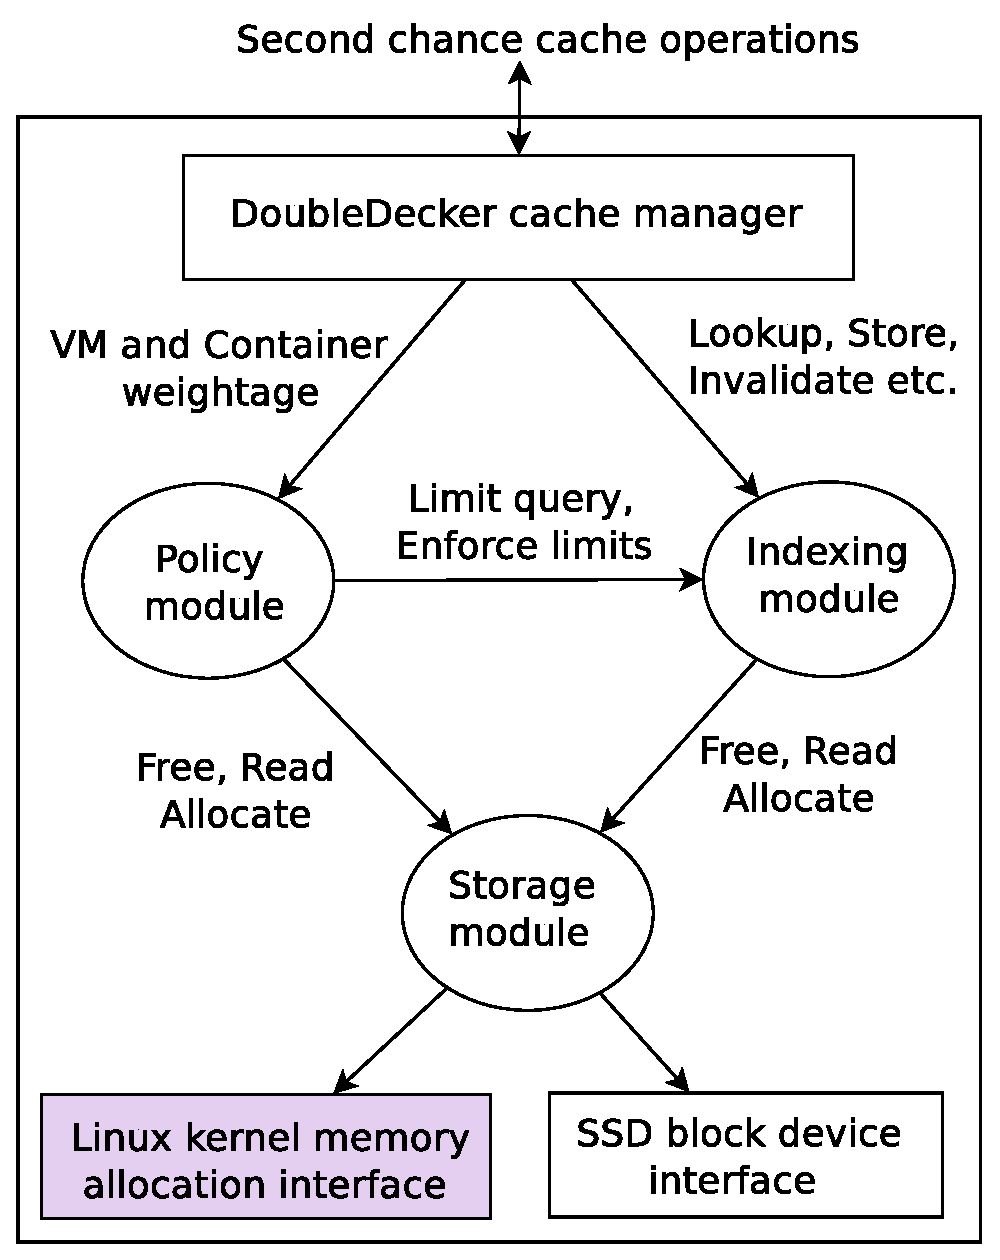
\includegraphics[width=0.33\textwidth]{images/ddecker} 
 \caption{\dd{} hypervisor cache components. 
% \puru{too many bidirectional arrows. Also naming
% consistency is required.}}
  }%
 \vspace{-0.5cm} 
 \label{fig:cachestore} 
\end{figure}
%
High-level design of \dd{} hypervisor cache store implementation 
is shown in Figure~\ref{fig:cachestore}.
%
The \dd{} cache manager interface is the entry point for all 
calls from the guest VMs (routed through the KVM hypervisor
cache interface) and configuration changes by the host administrator.
%\puru{cache access interface vs. hypervisor cache manager. i have
%used the latter a few times earlier.}
%

The host administrator may configure the memory size limits and SSD device 
limits for the \dd{} cache store which is handled by the
policy module.
%
Further, container level configurations explained before is
delegated to the policy module for cache management. 
%
On any configuration change, the policy module recalculates cache store
entitlements at two levels---per-VM level and container (pool) level.
%
The policy module monitors \dd{} cache usage by the VMs and containers and
takes appropriate action (e.g., eviction) when the cache entitlement is
violated.
%
In the current implementation, FIFO is used (LRU equivalent for exclusive caches)
to implement eviction at a pool level.

 
%

The indexing module is responsible for implementing normal second chance 
cache operations like lookup (\get), store (\put) etc..
% 
The key consisting of three tuples provided by the VM 
($<$\texttt{pool-id}{}$>$, $<$\texttt{inode-num}{}$>$, $<$\texttt{block-offset}{}$>$)
along with VM ID is used to map the request to storage objects.
%
A hierarchy of indexing data structures---per-pool file object (\texttt{inode-num}) hash 
table, file block radix-tree etc.---are used to map the key to a storage
object.
%
The opaque storage object is exchanged with the storage module
for actual storage operations.   
%
On a \put{} request, the indexing module enforces the limits by
checking the pool entitlement and evicting through the policy module,
if necessary.


Storage module provides backend independent services to 
read storage blocks, allocate new storage blocks and free storage blocks.
%
In the current \dd{} implementation, two types of storage backends are
implemented.
%
For memory storage backend, Linux kernel routines like \texttt{page\_alloc},
\texttt{page\_free}, \texttt{memcpy} etc. are used.
%
For SSD backend implementation, we have implemented a raw block device 
IO layer on top of the generic block device driver interface. 
%
The read calls (for \get{} operations) implements synchronous IO
operations while write calls (for \put{} operations) are implemented in an
asynchronous manner.

\subsection{\dd{} policy enforcement}

\begin{algorithm}[t]
  \caption{Victim selection from a list of cache using entities (VMs or Containers)}\label{algo:evict}
  \begin{algorithmic}[1]
    \Procedure{getvictim}{$Entities[1..n], EvictionSize$}\newline
      \Comment{\textit{EvictionSize}: \# of cached blocks to be evicted}\newline
      \Comment{\textit{Entities}: List of entities (VMs or containers)}
      \State \textit{overusedlist[1..n]}
      \State \textit{cumlweight} = 0
      \State \textit{underusedbuf} = 0
      \State \textit{count} = 0
      \For{i=1 to n}
          \State \textit{E$_i$} = \textit{Entities[i]}
          \If {\textit{E$_i$.entitlement} $<$ \textit{E$_i$.used + EvictionSize}} 
                 \State \textit{overusedlist[count]} = \textit{E$_i$}
                 \State \textit{cumlweight} += \textit{E$_i$.weightage}
                 \State \textit{count++}
          \EndIf
          \If {\textit{E$_i$.entitlement}-\textit{E$_i$.used}$>$2$*$\textit{EvictionSize}}
                 \State \textit{underusedbuf} += \textit{E$_i$.entitlement} - \textit{E$_i$.used} 
          \EndIf
      \EndFor
     \State \textit{E} = \textit{overusedlist[1]}
     \State \textit{exceedmax} = exceed(\textit{E}, \textit{underusedbuf}, \textit{cumlweight})
     \For{i=2 to count}
        \State \textit{E$_i$} = \textit{overusedlist[i]}
        \If {\textit{exceedmax} $<$ exceed(\textit{E})}
                    \State \textit{E} = \textit{E$_i$}
                    \State \textit{exceedmax} = exceed(\textit{E})
        \EndIf
     \EndFor
    \State Return E
    \EndProcedure
  \end{algorithmic}
  \label{algo:victim}
\end{algorithm}

%
To implement resource conservative cache management,
cached blocks are evicted only when the \dd{} cache limit is reached.
%
In such a case, selecting a victim application (container) is a two step process---first victim
VM is selected and then the victim container in the selected VM is 
decided.
%
Victim selection algorithm is same for both the levels (VMs and containers) and outline of 
the algorithm is presented in Algorithm~\ref{algo:victim}.
% 
The algorithm takes list of entities (VMs or Containers) and eviction size 
as input to return the victim entity.
%
List of entities who are over the limit of their entitlement---calculated directly
applying the \dd{} cache weightage configuration---are determined (line\# 8-12) and
stored in the \textit{overusedlist}.  
%
Sum of underutilized memory (\textit{underusedbuf}) is redistributed among
the entities as per their weightages to calculate their effective entitlements 
(\textit{E.entitlement} + (\textit{b} * \textit{E.weightage} / \textit{cw}))
and exceed values .
%
The exceed value for an entity is calculated as,
\begin{equation}
\begin{aligned}
exceed(\textit{E}, \textit{b}, \textit{cw}) = \textit{E.used} + \textit{EvictionSize} - \\
                                              (\textit{E.entitlement} + (\textit{b} * \textit{E.weightage} / \textit{cw}))
\end{aligned}
\end{equation}
where \textit{b} is the sum of under utilized entitlements (\textit{underusedbuf} in
Algorithm~\ref{algo:evict}), \textit{cw} is the sum of weightage percentage of entities whose cache
usage is above their respective entitlements.
%
The entity calculated with the highest exceed value is selected as the 
victim for eviction.
%
Only one victim entity is selected because 
we use a small batch (2MB) for eviction when a store request can not be
serviced because of global limit violations.

\begin{figure}[t]
\centering
\begin{subfigure}{0.38\textwidth} 
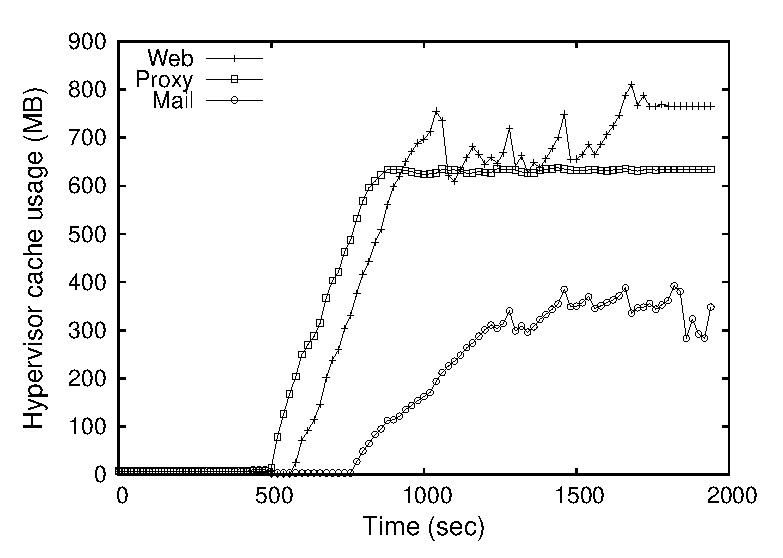
\includegraphics[width=\textwidth]{data/correctness/musage_global_new} 
 \caption{Global hypervisor cache (memory backed)}
 \label{fig:globalmem} 
\end{subfigure} 
%
\begin{subfigure}{0.38\textwidth}
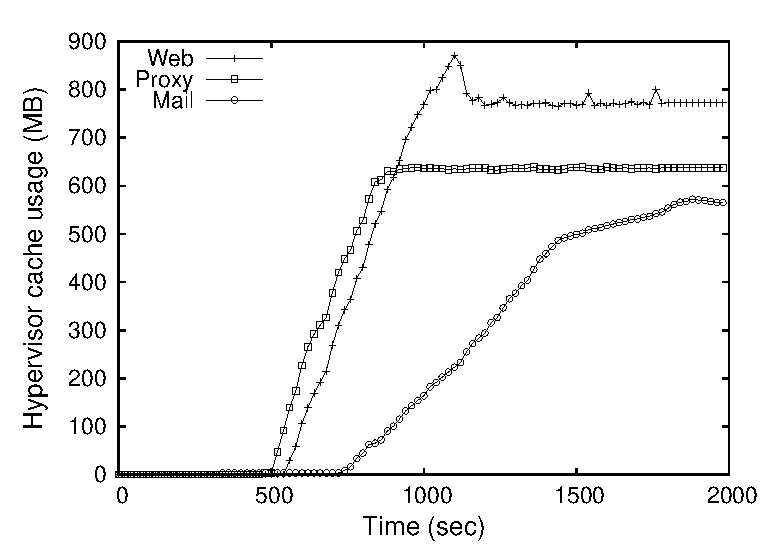
\includegraphics[width=\textwidth]{data/correctness/musage_ddecker_new} 
 \caption{\dd{} hypervisor cache (memory backed)}
 \label{fig:ddeckermem} 
\end{subfigure} 
%
\begin{subfigure}{0.38\textwidth}
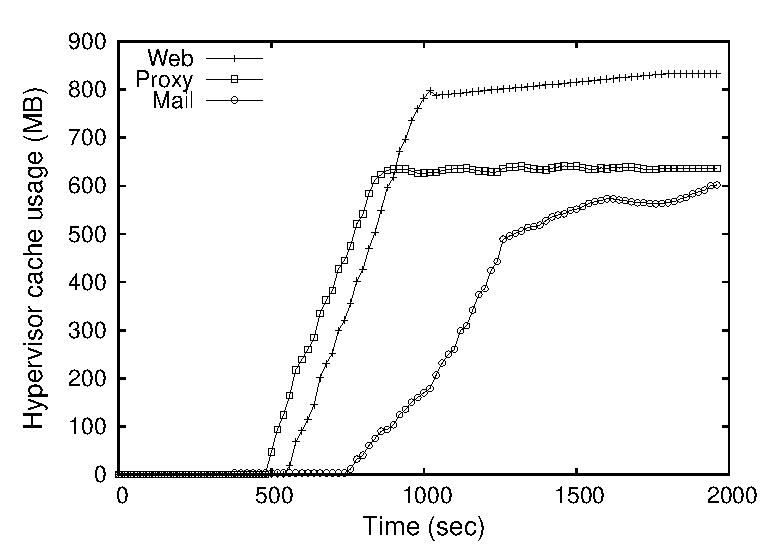
\includegraphics[width=\textwidth]{data/correctness/musage_global_ssd_new} 
 \caption{\dd{} SSD backed hypervisor cache}
 \label{fig:ddeckerssd} 
\vspace{-0.2cm}
\end{subfigure} 
%
\caption{Hypervisor cache distribution across application containers with
         different cache settings.}
\vspace{-0.25cm}
\label{fig:expt1}
\end{figure}
%{\bf Setup:} 

\section{Experimental evaluation}
\label{sec:expt}

The efficacy of \dd{} is established with a set of experiments using the
following setup,
a 16-core blade server with 3.4 Ghz  CPUs (Intel Xeon CPU E5-2650)
and 32 GB RAM.
%
A 240GB Kingston Digital SSDNow V300 SATA 3 solid state disk, accessed
through the SATA interface.
%
As workloads, we used
the \web, \proxy, \mail{} and \video{} profiles of the 
Filebench~\cite{filebench} workload suite.
%  
%

%\subsection{\dd{} cache size enforcement}
\subsection{Impact of caching modes}
The aim of this experiment is to establish correctness of the
two different cache store options of \dd, and to demonstrate the
benefits of partitioning the hypervisor cache.

\subsubsection{Cache size distribution}
For the experiment, a VM with 8 VCPUS and 8 GB RAM was used.
%
Four application containers (Container 1-4)  configured with 1GB RAM each,
executed the \web, \proxy, \mail, \video{} workloads.
%
All other resources (CPU and network) were allocated equally
across the application containers.  
%
Three hypervisor caching modes were compared---(i) a memory backed hypervisor cache 
with capacity 3 GB with global cache management mode, no
partitioning on a per-container basis (referred as \emph{Global}) % (\S Figure~\ref{fig:expt1}(a)), 
(ii) a 3 GB memory backed hypervisor cache with 
\dd{} cache management partitioning the cache equally among all containers
(referred as \emph{DDMem}),
%(\S Figure~\ref{fig:expt1}(b)), 
%cache management mode where every application container was assigned equal
%weightage of 25 
(iii) a 240 GB SSD backed hypervisor cache with 
\dd{} cache management partitioning the cache equally among all containers
(referred as \emph{DDSSD}),
%(\S Figure~\ref{fig:expt1}(c)). 
%cache management parwith equal weightages for each application container.
%weightage of 25 (\S Figure~\ref{fig:expt1}(c)). 
% 

\begin{figure}[t]
  \centering
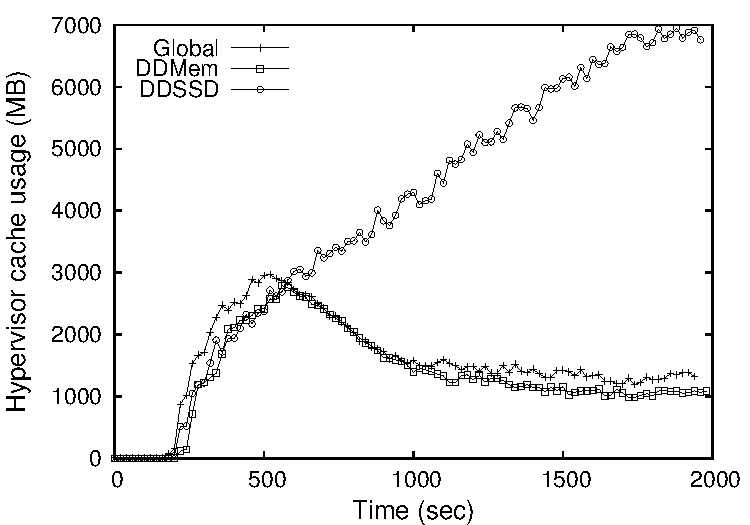
\includegraphics[width=0.38\textwidth]{data/correctness/only_video}
 \caption{\dd{} cache usage by \video-workload with different cache
          configurations.}
 \vspace{-0.5cm}
 \label{fig:video}
\end{figure} 



\begin{table*}[t]
\scriptsize
\begin{center}
\begin{tabular}{|c|c|c|c|c|c|c|c|c|c|c|c|c|}
\cline{2-13}
\multicolumn{1}{c}{} & \multicolumn{4}{|c|}{\bf Global (Memory)} & \multicolumn{4}{c|}{\bf DoubleDecker (Memory)} & \multicolumn{4} {c|}{\bf DoubleDecker (SSD)}\\
\cline{1-13}
\multicolumn{1}{|c|}{} & {\bf Throu-} & {\bf Latency} & {\bf lookup-} & {\bf \# of} & {\bf Throu-} & {\bf Latency} & {\bf lookup-}&{ \bf \# of} & {\bf Throu-} & {\bf Latency} & {\bf lookup-} & {\bf \# of}\\
%
\multicolumn{1}{|c|}{} & {\bf ghput} & {\bf (ms)} & {\bf to store} & {\bf evic-} & {\bf ghput} & {\bf (ms)} & {\bf to store}& {\bf evic-} & {\bf ghput} & {\bf (ms)} & {\bf to store} & {\bf evic-}\\
%
\multicolumn{1}{|c|}{\bf Workload} & {\bf (MB/s)} & & {\bf ratio (\%)} & {\bf -tions} & {\bf (MB/s)} & & {\bf ratio (\%)} & {\bf -tions} & {\bf (MB/s)} & & {\bf ratio (\%)} & {\bf -tions} \\
\hline
\hline
\web & 14.2 & 29.2 & 93 & 209815 & 93.7 & 3 & 99 & 0 & 5.5 & 73 & 91 & 0 \\
\hline
\proxy & 5.4 & 89.1 & 76 & 2880 & 5.6 & 85.9 & 76 & 0 & 5.2 & 91.5 & 75.9 & 0\\
\hline
Mailserver & 1.3 & 598.2 & 1 & 159793 & 1.4 & 555.7 & 32 & 0 & 2 & 386.7 & 44 & 0\\
\hline
\video & 1276 & 2.6 & 65 & 1650424 & 1188 & 2.9 & 57 & 2076672 & 481.5 & 7.8 & 67 & 0 \\
\hline
\end{tabular}
\caption{Application performance and cache behavior comparison with 
         different hypervisor caching schemes.}
\vspace{-0.7cm}
\label{table:hcache}
\end{center}
\end{table*}


Hypervisor cache distribution across the containers executing the \web, \proxy{} 
and \mail{} workloads with different caching configurations is 
shown in Figure~\ref{fig:expt1}.
%
The \video{} workload dominated the cache usage; for better presentation
cache usage of the \video{} workload with different caching modes is shown
in Figure~\ref{fig:video}.
%
As can be seen from Figure~\ref{fig:expt1} and Figure~\ref{fig:video}, 
for the first 500 seconds there is no requirement of the hypervisor cache
except for the \video{} workload. During this duration, container with
the \video{} workload occupies up to 3 GB of the cache (in all caching modes).
Beyond 500 seconds, the memory requirements of other workloads also
do not fit in the VM and the corresponding containers 
contend for the second chance cache.
Correspondingly, the \video{} workloads cache occupancy decreases from 3 GB to 1.4 GB.

With the global cache policy, there is no deterministic cache capacity 
for each container and all four workloads contend for the cache.
The result cache size distribution for each workload is dependent
on its access patterns and the access rate. Since \video{} workload
has the higher IO rate and quantity, it still consumes the largest
portion of the cache. The cache of the \web{} and \mail{} workloads
gets affected the most, as objects of these containers are evicted
from the cache due to pressure from the other two workloads.
In fact, the \mail{} workload gets a maximum share of less than 400 MB,
as against its fair share of 750 MB.

%With global hypervisor caching (Figure~\ref{fig:globalmem}, Figure~\ref{fig:video}), 
%\video-workload reached a cache usage peak of 
%3GB and came down to around 1.4 GB when other workloads started contending
%for the cache.
%
With \dd{} equal-weight cache partitioning (Figure~\ref{fig:ddeckermem}), 
the \video-workload was allocated ~1.2 GB when other workloads started 
using the cache up to their own entitlements. 
Since, the \proxy{} and \mail{} workloads did not consume their 
entire share of 750 MB,
the remaining capacity was shared between the \video{} and \web{} workloads.
In fact the \web{} workload does not consume more than 800 MB and hence
~1.2 GB is consumed by the \video{} workload.
%
Note that with \dd{} mode, cache usage of workloads other than \video-workload 
did not take any dips once they reached their respective peaks as opposed to
global mode.
%
This demonstrates {\em resource conservative nature} of \dd{} 
cache provisioning with {\em guaranteed isolation} according
to assigned priorities.
%
With SSD backed hypervisor caching (Figure~\ref{fig:ddeckerssd}), the cache 
size was sufficient to for all the workloads. This verified two things,
one the \dd{} could manage a SSD-based cache store correctly and
second the peak cache usage in the DDMem caching mode.
%
%So, the cache usage behavior was same with global mode and \dd{} eviction
%mode.


\subsubsection{Performance impacts with caching modes}
%Impact of cache distribution changes is shown in Table~\ref{table:hcache}.
The impact of cache distribution with different caching modes
is reported in Table~\ref{table:hcache}.
%
\web{} throughput with the DDMem caching mode (\dd{} with in-memory cache store)
was approximately {\em six times} better than the global caching mode.
%
With the \dd{}  DD-mem caching mode, \mail{} and \proxy{} workloads resulted
in marginal improvements ($\sim$5\%) and the \video-workload resulted 
in small degradation ($\sim$6\%) in application performance.
%
With the global eviction mode, evictions from workloads other than
\video{} were noticed, e.g., $\sim$200K evictions from the \web{} container. 
%
With \dd, only the \video-workload was victimized to enforce
equity at the container-level according to the equal cache distribution
configuration.

No evictions were noticed with the SSD-backed hypervisor cache % because
as the cache could host all disk cache blocks for all the
containers.
%
Because of the increased IO latency of SSD access, application
throughput for the \web{} and \video{} workloads 
was around 300\% lower compared to memory backed hypervisor cache.
%\puru{not sure how to interpret 300\% decrease.}
%\puru{to replace---decreased by 90\% and 60\% respectively.}
%
Interestingly, throughput and latency of \mail{} workload improved
by 30\% and 40\%, respectively.
%
This is due to offloading of disk operations of other workloads 
through sufficient SSD availability in the hypervisor cache.
%
These results show that even in case of sufficient hypervisor cache
availability, enforcing fairness across applications can result in
significant application benefits.


\subsection{Flexible hypervisor cache management}
\label{subsec:flex}
%
\begin{table}[t]
\scriptsize
\begin{center}
\begin{tabular}{|c|c|c|c|c|}
\hline
{\bf Cache} & {\bf Webserver} & {\bf Proxycache} & {\bf Mail} & {\bf Videoserver} \\
{\bf Setting} & {\bf (C1)} & {\bf (C2)} & {\bf (C3)} & {\bf (C4)} \\
\hline 
\hline 
DDMem & Mem: 32 & Mem: 25 & Mem: 25 & Mem: 18 \\
DDMemEx & Mem: 40 & Mem: 30 & Mem: 30 & Mem: 0 \\
DDHybrid & Mem: 40 & Mem: 30 & Mem: 30 & SSD:100 \\
\hline 
\end{tabular}
\caption{\dd{} cache configuration settings.}
\vspace{-1cm}
%\puru{in previous experiment mentioned as DD-mem,etc. Fix formatting}}
\label{table:settings}
\end{center}
\end{table}
%
To analyze the effectiveness of container level priority extensions to the 
hypervisor caching, we have performed an experiment with application containers
configured with different memory limits.
%
In this experiment, the \web{} container (C1) was configured with a memory 
limit of 1.25 GB (through \cgroups) and the \video{} container (C4) was configured 
with a memory limit of 750 MB.
%
Other two containers were configured with 1 GB memory limit each.
%
The \dd{} memory cache size was limited to 2 GB.
%2 GB limit was set to the total \dd{} memory cache size,
%%which was shared by all
%the applications.
%   
In the global eviction mode (referred to as Global), only the container 
level memory limits were in action while the \dd{} hypervisor cache was 
shared globally without any container-level priority enforcement.
%
Three different cache settings (DDMem, DDMemEx and DDHybrid), shown in 
Table~\ref{table:settings}, were used to partition the \dd{} hypervisor cache
across the application containers.
%
The DDMem policy extended the \cgroup{} level memory allocation weights to the
\dd{} hypervisor cache.
%
The DDHybrid policy used the SSD store for the \video{} workload, while
containers C1-C3  shared the memory cache with weights 40, 30 and 30, respectively.
\begin{figure}[t]
  \centering
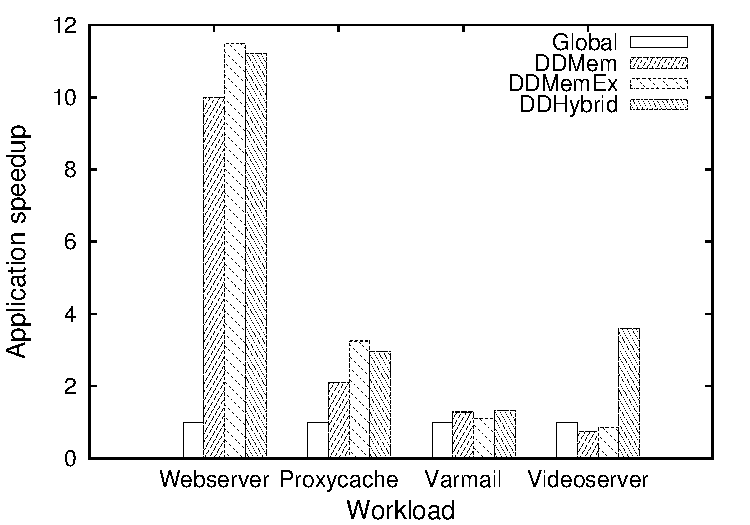
\includegraphics[width=0.43\textwidth]{data/singlevm_policy/speedup}
\vspace{-0.2cm}
 \caption{Comparison of application performance with differentiated 
          hypervisor caching policies vs. global hypervisor cache
          management.}
 \label{fig:policy_speedup}
\vspace{-0.4cm}
\end{figure} 
\begin{figure}[t]
\centering
\begin{subfigure}{0.38\textwidth} 
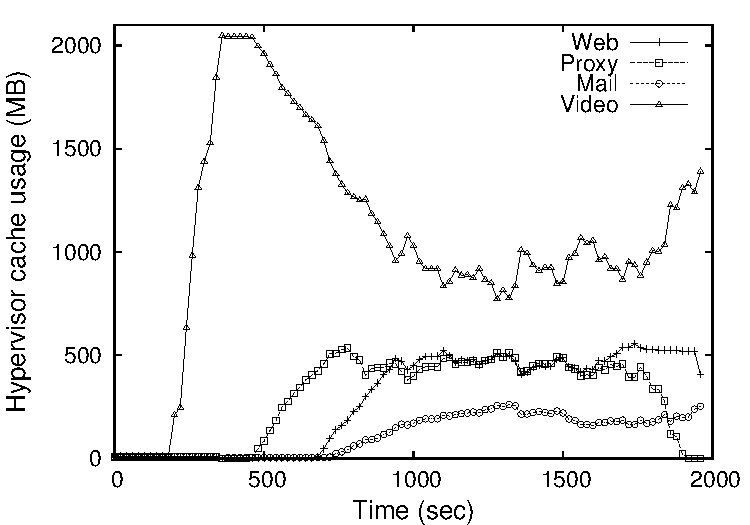
\includegraphics[width=\textwidth]{data/singlevm_policy/musage_global} 
 \caption{Global hypervisor cache}
 \label{fig:gmem1} 
\end{subfigure} 
%
\begin{subfigure}{0.38\textwidth}
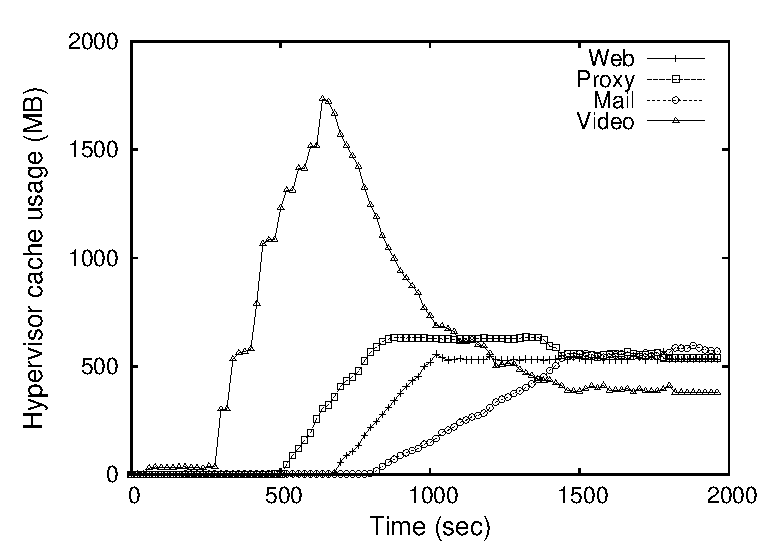
\includegraphics[width=\textwidth]{data/singlevm_policy/musage_dd_mem} 
 \caption{DDMem \dd{} policy}
 \label{fig:ddmem} 
\end{subfigure} 
%
\begin{subfigure}{0.38\textwidth}
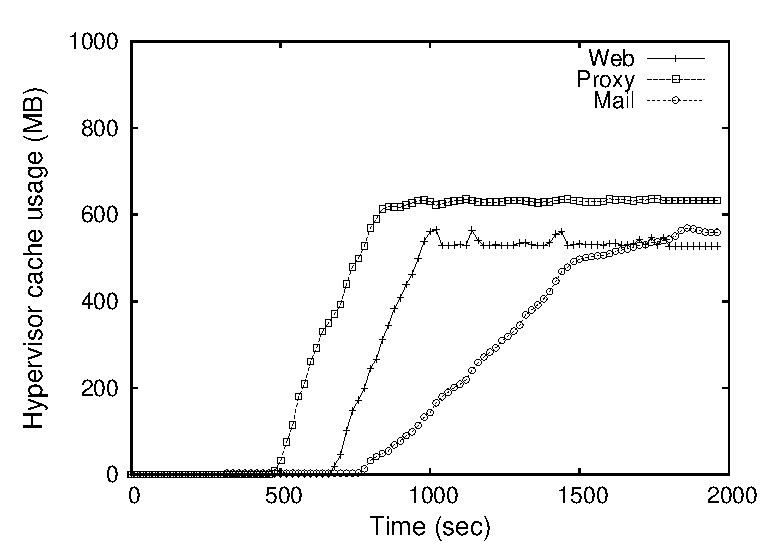
\includegraphics[width=\textwidth]{data/singlevm_policy/musage_dd_hybrid} 
 \caption{DDHybrid \dd{} policy}
 \label{fig:ddhybrid} 
\vspace{-0.2cm}
\end{subfigure} 
%
\caption{Hypervisor cache distribution across application containers with
         different cache management policies.}
\vspace{-0.7cm}
\label{fig:expt2}
\end{figure}

Application throughput improvements w.r.t the global hypervisor 
cache management mode 
and the different \dd{} caching policies is shown in Figure~\ref{fig:policy_speedup}.
%\puru{maybe unified is better than global.}
%
For the \web-workload, significant application throughput improvement
was observed---10x, 11x and 11x compared to global caching with
DDMem, DDMemEx and DDHybrid policies, respectively.
%
Around 2x, 3.2x and 3x application performance improvement resulted 
for the \proxy-workload with the three \dd{} caching modes.
%DDMem, DDMemEx and DDHybrid
%policies, respectively.
%
With the \mail{} workload, the application performance gains were marginal.
%
With the \video-workload application performance decreased with
the DDMem ($\sim$25\%) and DDMemEx ($\sim$20\%) caching modes
compared to that of the Global mode.
%
This was because the application's aggressive hypervisor cache usage 
behavior was curtailed by \dd{} policies.
%
When the \video-workload's hypervisor cache was moved to the SSD, 
3.6x improvement in application throughput was observed
compared to the global mode caching mode.

 

Hypervisor cache distribution across application containers
with the different caching modes 
as shown in Figure~\ref{fig:expt2}.
%
With the global mode, the hypervisor cache usage was dominated by the \video-workload
while other applications (C1-C3) contended for the cache
and could never reach a proportionate sharing ratio.
%
With\dd's DDMem policy, cache usage of \video-workload reduced to 
the minimum (around 400 MB), close to its fair share,
when other applications started using the cache.
%
Memory cache usage by the \web, \proxy{} and \mail{} workloads is shown in 
Figure~\ref{fig:ddhybrid} when hypervisor cache for the \video-workload 
was moved to the SSD cache (the DDHybrid mode). 
%
In this case, the 2 GB memory available for the memory backed
region of the \dd{} hypervisor cache
%configured memory backed cache of size 2GB 
was sufficient to serve all the application without resulting in 
any evictions. The three containers, each occupied about 500 MB to 600 MB
of the cache.

The main take-away from this experiment was that usage of the hypervisor cache
for different applications can be configured carefully, either to use
the memory store or the SSD store, for positive benefits for all applications.

%\puru{move figure 11 to single row.}
\subsubsection{Efficacy of cooperative memory management}
\label{subsec:coop}

%\begin{table}[t]
%\small
%\begin{center}
%\begin{tabular}{|c|c|c|c|}
%\hline
%{\bf Workload} & \bf{Technique} & {\bf Through-} & {\bf Memory} \\
% & & {\bf put (ops/sec)} & {\bf usage (GB)} \\
%\hline 
%\hline 
%{\bf MongoDB} & Morai++ & 16.9 & 0.5,1.3 \\
%%\cline{2-4}
%{\em (15 ops/sec)} & DD & 25.1 & 1,0.4 \\
%\hline
%{\bf Webserver} & Morai++ & 1289 & 2.2,0.5 \\
%%\cline{2-4}
%{\em (800 ops/sec)} & DD & 988 & 1,1.6 \\
%\hline
%{\bf Redis} & Morai++ & 13 & 1.8, 0 \\
%%\cline{2-4}
%{\em (5000 ops/sec)} & DD & 11186  & 2,0 \\
%\hline
%{\bf MySQL} & Morai++ & 48.5 & 1.6,0 \\
%%\cline{2-4}
%{\em (100 ops/sec)} & DD & 132.7 & 1.9,0 \\
%\hline 
%\end{tabular}
%\caption{\dd{} vs. centralized second chance cache management}
%\vspace{-0.5cm}
%\label{table:ddsdc}
%\end{center}
%\end{table}

\begin{table}[t]
\small
\begin{center}
\begin{tabular}{|l|c|c|c|}
\hline
{}           & {} & {} & {App. memory,}\\
{ Workload}  & { Technique} &  Throughput{} & {Hypervisor} \\
{\em (SLA)} & & { } & {cache}  \\
& & { (ops/sec)} & {(GB)}  \\
\hline 
\hline 
{\bf MongoDB} & Morai++ & 16.9 & 0.5, 1.3 \\
%\cline{2-4}
{\em (15 ops/sec)} & \dd{}& 25.1 & 1, 0.4  \\
\hline
{\bf MySQL} & Morai++ & 48.5 & 1.6, 0 \\
%\cline{2-4}
{\em (100 ops/sec)} & \dd{} & 132.7 & 1.9, 0 \\
\hline
{\bf Redis} & Morai++ & 13 & 1.8, 0 \\
%\cline{2-4}
{\em (5000 ops/sec)} & \dd{} & 11186  & 2, 0 \\
\hline
{\bf Webserver} & Morai++ & 1289 & 2.2, 0.5 \\
%\cline{2-4}
{\em (900 ops/sec)} & \dd{} & 988 & 1, 1.6  \\
\hline 
\end{tabular}
\caption{Comparison of centralized second chance cache management with \dd{}.}
\vspace{-1cm}
\label{table:ddsdc}
\end{center}
\end{table}
%To demonstrate the effectiveness of \dd{} 
%in ensuring application performance guarantees and improve overall system-wide
%performance, we performed the following experiment.
%
\dd{}, with its cooperative memory management framework, can explore 
holistic provisioning solutions that traditional centralized hypervisor
based techniques cannot.
%
To demonstrate such capabilities, we performed the following experiment.
%
A single VM hosted four application containers and executed the 
MongoDB, Redis, MySQL data stores and the Filebench webserver workload.
The data stores acted as backends for YCSB clients.
%and
%MySQL workloads with 
The VM was provisioned with 6GB memory and 8 CPUs (2 CPUs pinned
to each application container).
%
The hypervisor cache was provisioned to 2GB.
%
To approximate a centralized hypervisor cache management approach 
like Morai~\cite{sdc},
we iterated over different cache partitions at the hypervisor 
cache and report
results of the best configuration (referred to as Morai++).
%
Each application had a target throughput SLA to achieve (mentioned
in the first column of Table~\ref{table:ddsdc}). The best configuration
was the one which met the individual application SLAs and yielded
the maximum aggregate throughput.
%
%we tried different cache partitioning at the hypervisor level while the VM level
%memory provisioning was left untouched.
% 

Referring to Table~\ref{table:ddsdc}, a hypervisor cache partition of 60:40 
between the MongoDB workload and the Webserver workloada met their SLA requirements
and yielded the maximum aggregate throughput with Morai++.
%
Morai++ could not satisfy application performance targets of Redis and MySQL 
workloads while barely managed to meet MongoDB performance targets. 
%
In this setup, usage of the 6GB VM memory (shared
by all containers) was 0.5 GB, 1.6 GB, 1.8 GB and 2.2 GB, for the 
MongoDB, MySQL,
Redis and Webserver workloads, respectively.
%
%The best hypervisor cache partition (referred to as Morai++)
%---adherence to minimum individual application 
%performance (Table ~\ref{table:ddsdc}, column 1) with maximum 
%global performance---is compared 
%against the best \dd{} provisioning option (referred to as DD in Table~\ref{table:ddsdc}). 
%
%when cache was partitioned in the ratio of 60:40 between MongoDB and 
%Webserver applications. 
%\puru{does not look like 60:40 in the table.}
Interestingly, with Morai++, actual hypervisor cache usage was not in the ratio of 60:40
and total average usage was below 2 GB (~1.8 GB).
%
%
%
%In all other cases of higher share allocation to MongoDB, there was no noticeable performance
%improvements for MongoDB.
%
%The average memory usage for different applications is presented in the form \textit{X,Y} in 
%Table~\ref{table:ddsdc}, where \textit{X} represents in-VM memory usage and \textit{Y} represents
%hypervisor cache usage.  
%
This was because the Webserver workload dominated the in-VM memory usage 
and did not need its maximum share of hypervisor cache leaving MongoDB-workload
to use the residual amount as per its demand (See Algorithm~\ref{algo:victim}).
%
The MongoDB workload (throttled inside the VM) could not leverage the
maximum possible hypervisor cache usage. 
%
As an additional effect, the in-VM memory usage dominance of the Webserver-workload
adversely affected other applications, notably Redis whose
working set size was ~2 GB and which did not fit in memory.
%
Note that, both Redis and MySQL applications are designed
to work only with anonymous memory and did not use the hypervisor cache
integrated with the file IO path.
%
%
%(in-VM memory) causing other
%applications to starve for memory which can not be helped by any cache partitioning scheme
%employed by Morai++.
%
With \dd{}, the VM-level manager can incorporate this information to
provision memory both from the VM and the hypervisor cache which
%
%This the main feature
the centralized hypervisor caching techniques lack. 
%
In our experiment, with \dd{}, we configured the VM memory to be allocated
as 1 GB, 2 GB, 2 GB and 1 GB, for the MongoDB, MySQL, Redis, and Webserver
workloads, respectively and discovered the best hypervisor cache
partition.
%
Based on this setup, \dd{} meets the application SLA requirements
of all the applications and the aggregate throughput achieved is higher
by a large margin.
%
This achieved primarily through improvements in the throughputs achieved
by the MySQL and Redis applications.
%
Note that, both these memory-bound applications were positively 
benefited by \dd{}.
%
Also, since the working set of Redis could be accommodated in memory,
its throughput increased by a factor of 1000.


%On the other hand, 
Based on the above results, 
we demonstrate that two-level provisioning capability of \dd{} enables
holistic memory configurations which can account for application
characteristics and requirements, and yield improved application-level
and system-wide performance.
%
For workload provisioning in an adaptive manner,
\dd{} can employ well known techniques like MRC~\cite{mrc,membal},
 WSS estimation~\cite{wss,wsslow}, SHARDS~\cite{shards} etc..
%
Note that, the estimation should be done from within the VM which allows the
guest OS memory manager to provision memory resources at the two levels.
%
Centralized nesting agnostic hypervisor cache management techniques
cannot explore such provisioning configurations.
%
%space over the two levels (in-VM memory and hypervisor cache memory),
%the DD policy could meet individual application performance targets and resulted in 
%maximum system-wide benefits. 
%
\subsection{Dynamic cache management}
\begin{figure}[t]
  \centering
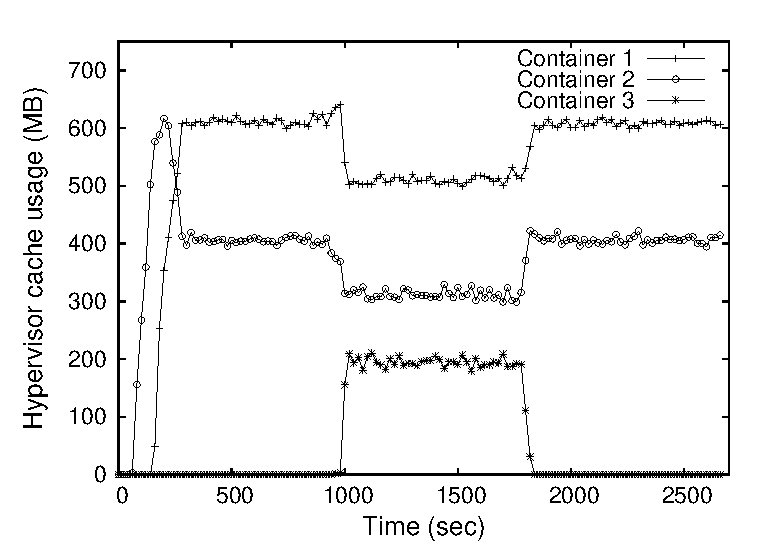
\includegraphics[width=0.38\textwidth]{data/dynamic_containers/musage}
\vspace{-0.2cm}
 \caption{Dynamic policy changes with \dd{} cache and its impact on cache 
          distribution across containers.}
\vspace{-0.55cm}
 \label{fig:dyn_distrib}
\end{figure} 
%
To demonstrate \dd's capability to apply dynamic hypervisor cache
partitioning across containers and virtual machines, we performed the
following experiments.
%
\subsubsection{Dynamic management across containers}
Initially, a single VM was configured with two application containers.
%
%
A 1 GB memory limit was configured for \dd{} memory cache while 
the SSD cache size was 240 GB.
%
Container 1 and 2 were configured with 1 GB memory each in the
virtual machine and 
executed the \web{} and \proxy{} workloads, respectively.  
%
The \dd{} cache distribution weights 
for Container 1 and 2 were set to 60 and 40, respectively.
%
After 900 seconds into the experiment, a third container (Container 3) was booted 
which executed the \video-workload.  
%
At this point, the \dd{} cache distribution weights were configured as
50, 30 and 20 for Containers 1-3, respectively.
%
After continuing with this setting for 900 seconds, the 
\video-workload (Container 3)
was configured to use the SSD store for its hypervisor cache and 
the share of Container 1 and 2 for the memory store
was reset to 60 and 40, respectively.

The \dd{} memory cache allocation across the three containers is as shown 
in Figure~\ref{fig:dyn_distrib}.
%
Initially, the cache allocation for Containers 1 and 2 were approximately 
600 MB and 400 MB,
respectively.
%
At around 1000 seconds from the start of the experiment, the \dd{} cache got 
redistributed---$\sim$500 MB for Container 1, $\sim$300 MB  for Container 2 and
$\sim$ 200 MB for Container 3---when Container 3 started using its cache entitlement.
%
Finally, when the \dd{} cache setting for Container 3 was dynamically changed 
from memory to SSD (at around 1800 seconds), the hypervisor memory 
cache was re-distributed in the ratio of 60:40 between Container 1 and Container 2.
%
Container 3 used the SSD backed \dd{} cache for the rest of the 
experiment (not shown in Figure).
%
\dd's support for dynamic cache partitioning policies provides
flexibility in designing higher level memory management solutions. 

\subsubsection{Dynamic management across virtual machines}
\begin{figure}[t]
  \centering
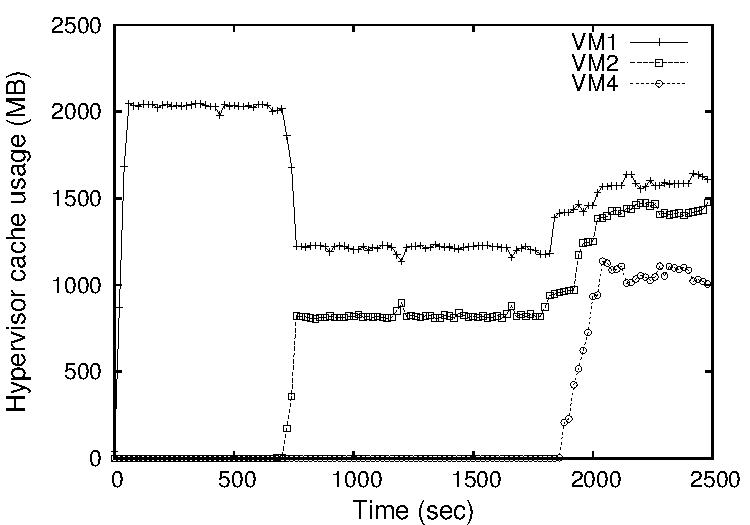
\includegraphics[width=0.38\textwidth]{data/dynamic_vms/musage}
\vspace{-0.2cm}
 \caption{Dynamic VM provisioning with policy changes triggering \dd{} cache 
          redistribution across VMs.}
\vspace{-0.25cm}
 \label{fig:vm_distrib}
\end{figure} 
In a dynamic VM provisioning setup, the number of VMs and resources
available for each change with time.
%
To demonstrate \dd's suitability in this setup, we performed the
following experiment.
%
Four VMs, each configured with 4GB RAM were started at an
interval of 600 seconds and
each executed the \video{} workload within 
a single application container. 
%
Initially, the \dd{} memory backed cache size limit was 2 GB and VM1 
was given a weightage of 100.
%
When VM2 boots up (at 600 seconds), the \dd{} cache weights 
for VM1 and VM2 were set to 60 and 40, respectively.
%
VM3 was only allowed to use the SSD cache when it started at around 1200 
seconds; VM1 and VM2 cache settings remained the same.
%
At around 1800 seconds from the start of the experiment, another
virtual machine VM4 was started.
and the \dd{} memory backed cache size was increased to 4 GB.
%
Further, the cache distribution weightages for VM1, VM2 and VM4 
were configured as 40, 35 and 25, respectively.

\dd{} cache distribution across VM1, VM2 and VM4 is as shown in
Figure~\ref{fig:vm_distrib}.
%
VM1 used up the \dd{} cache entirely (2 GB) until VM2 started
using the cache (at around 650 seconds) when the cache share of
VM1 and VM2 became $\sim$1200 MB and $\sim$800 MB, respectively.
%
Instantiation of VM3 (at around 1800 seconds) did not disturb the cache
distribution between VM1 and VM2 as VM3 used the SSD cache (VM3 usage
not shown in Figure). 
%
Finally, when VM4 started and the cache capacity of \dd{} was changed 
along with cache partitioning weights, 
average cache usage of VM1, VM2 and VM4 was  
around 1600 MB, 1400 MB and 1000 MB, respectively.


With these two experiments, we demonstrated the capability of \dd{}
to dynamically manage two-levels of cache specifications in a
dynamic manner. Policy decision at the hypervisor which effect
VM-level cache partitioning and decisions that effect the
per-container partition sizes for each VM can be handled by \dd{}
in a dynamic manner. This feature is a key enabler to develop
adaptive memory and cache management policies depending
on application behavior, workloads and execution entity priorities.


\section{Related work}
\label{sec:related}
\noindent
{\bf Hypervisor caching:} A hosted virtualization solution like 
KVM~\cite{kvm, kvmconfig} naturally offers \emph{inclusive}
hypervisor caching by virtue of being in the disk access path.
%
Singleton~\cite{singleton} performs cache translation of the
inclusive hypervisor cache to provide exclusive caching by deduplicating
KSM scanned pages and the inclusive cache.
%in an indirect manner.
%
Transcendent memory~\cite{memtrans} proposed a guest OS supported
exclusive caching framework which was
first implemented in Xen~\cite{oracletmem}.
%  
Exclusive hypervisor cache for KVM ~\cite{kvmzcache} based on the 
transcendent memory model enabled several caching combinations and 
%is comparatively
%analyzed to study the effectiveness of the hypervisor caching solutions.
analyzed effectiveness of the hypervisor caching solutions.
%  
All of the above solutions provide hypervisor cache management capability
at a VM granularity whereas \dd{} extends the framework to support application
level differentiated hypervisor cache partitioning in derivative
cloud setups.
%like for
%application containers hosted inside the VMs.
%
Mortar~\cite{mortar} exposed the hypervisor cache to distributed memory store 
applications like \textrm{memcached}~\cite{memcached} by modifying the application in an
explicit manner.
%
Our approach is more generic and does not require any modifications to 
applications.
%
Software-defined caching ~\cite{sdc} proposed application SLA guided 
dynamic second chance inclusive cache provisioning by hosting applications 
on separate virtual disks.
%
\dd{} provides additional flexibility in terms of hypervisor cache provisioning
with exclusive cache support and by providing different second chance storage options.
%
Moreover, our approach is better equipped to meet the decentralized memory 
management requirements of a derivative cloud setup as shown 
in \S\ref{subsec:sdc} and \S\ref{subsec:coop}.
%while the approach in ~\cite{sdc} is proposed for 
%multi-VM setups, we believe that the approach is in-principle 
%applicable to application containers as well;
%we provide a realization of the same. 

\noindent
{\bf Application containers and derivative clouds:} Linux \cgroups~\cite{cgroup},
BSD jails~\cite{jail} and Solaris Zones~\cite{zone} provide operating system 
level isolation support for different applications.
%  
LXC~\cite{lxc} and Docker~\cite{docker} are two popular application container
enablers built by exploiting the Linux \cgroup{} resource control framework.
%
Nested virtualization~\cite{turtle,blanket,recursv} enables hosting VMs inside a VM
by exposing hardware virtualization features to the first level VM.
%
The goal of nested virtualization has been to address security issues~\cite{vx32},
VM standardization related problems and hypervisor trouble-shooting. 
%
Resource management in nested virtualization setups has been proposed 
by ~\cite{intercloud} and ~\cite{supercloud}.
%
Intercloud~\cite{intercloud} and Supercloud~\cite{supercloud} propose 
interoperable 
cloud services 
decoupled from the cloud provider. 
%\puru{Add a line about intercloud and supercloud functionality}.
%by inter-clouds~\cite{intercloud} and super-cloud~\cite{supercloud}.
%
Derivative clouds in the current era~\cite{spotcheck, heroku, picloud} use 
containers inside the VMs as the IaaS primitive because virtualization 
overheads using containers is significantly lower than 
nested VM virtualization.
%
\dd{} enhances the provisioning flexibility through hypervisor cache management
at the nested container level and opens up resource-based SLA
business model enhancements for 
derivative clouds.


\noindent
{\bf Memory management in virtualized systems:} Memory 
ballooning~\cite{vmware,hotplug} facilitates dynamic adjustment of VM memory  
allocations.
%
Several dynamic ballooning based controllers to estimate and adjust the memory 
allocation to the VMs have been proposed~\cite{wss, membal, tws}.
%
Hypervisor caching and \dd{} complements the dynamic memory controllers
by providing symbiotic resource management capabilities.
%
\dd{} extends the flexibility of memory resource management in container 
within VM setups.
%
Memory deduplication~\cite{vmware,ksmpaper,satori} is another memory
efficiency enhancement technique shown to be useful in virtualized
systems~\cite{ksmpaper,utc}.   
%
Integration of \dd{} with deduplication to enhance the memory management
efficiency in a derivative cloud setup would be an interesting future
direction of our work.
%\puru{can we add another line about what this integration would mean,
%or what it implies for design? this is preceding line.}
%
%\revised{
While deduplication of hypervisor cache itself can be easily incorporated
into \dd{}, deduplication across hypervisor cache and memory used by VMs requires
additional techniques.
%While exclusive caching takes care of deduplication of objects in
%%of memory across 
%the hypervisor cache and page cache of individual virtual machines, there is 
%a chance of content duplication across virtual machines and the hypervisor
%cache.
%
Synergy~\cite{synergy}, a holistic deduplication technique in virtualized systems,
combines benefits of sharing and ballooning for resource provisioning
via the hypervisor cache. 
%
%\deba{cant comprehend the next sentence}
With the two-level storage option of \dd{}, 
shareable and non-shareable pages can use different storage options
to improve performance. We see this as yet another complimentary 
direction for future work.
%}
%to different treatment of shared and unshared pages, and is yet another
%interesting direction of future work.
%
% can be 
%incorporated into DoubleDecker to address the issue of duplication and left as
%a future direction. 
%}
%


\section{Conclusions}
%
Popularity of low-overhead application container 
frameworks has enabled derivative cloud based
business models.
%
Several challenges in efficient resource management 
for nested (containers inside VMs) setups require rethink
of existing designs.
%
In this paper, we proposed \dd, a cooperative memory
management framework which enabled multi-level provisioning
of VM-level memory and the hypervisor cache.
%resource conservative 
%memory management along with guaranteed container level
%isolations.
%
%\dd{}, an application container aware hypervisor cache provisioning
%mechanism,
%provides flexible memory management options and differentiated
%memory provisioning at multiple levels.
%
%
\dd{} supports two storage backends i.e., memory and SSD,
and provisioning configurations at two levels---per-VM and 
per-application container, for adaptive provisioning.
%
Our experimental evaluation demonstrated the effectiveness of
\dd{} % by improving application performance 
by extending container level priorities to the hypervisor cache.
%
We also showed that selective usage of different storage
options of the hypervisor cache 
based on application characteristics,
improved overall performance in the derivative setup.
%
%Selective provisioning of applications on the SSD backend
%is beneficial for all applications hosted in the derivative setup.
%
Most importantly, \dd{} 
can simultaneously provision memory at the VM-level and the hypervisor cache,
and effectively meet requirements of decentralized memory management
in derivative cloud setups.
%to address 
%decentralized memory management requirements of 
%a derivative cloud
%setup which existing solutions do not address sufficiently.
%
%While \dd{} tested simple illustrative policies, 
%we believe our work can facilitate sophisticated 
%usage of policies that can handle multiple levels
%of priorities and multiple storage backends.



\section*{Acknowledgements}
We would like to thank our shepherd, Akshat Verma,
and the anonymous referees for their helpful comments.
\bibliographystyle{acm}
\bibliography{ddecker}

\end{document}
